
\documentclass[a4paper,11pt]{article} % тип документа
%\usepackage{jmlda}

% Рисунки
\usepackage{graphicx}
\usepackage{wrapfig}
\graphicspath{ {./images/} }

\usepackage{hyperref}
\hypersetup{				% Гиперссылки
    colorlinks=true,       	% false: ссылки в рамках
	urlcolor=blue          % на URL
}


%  Русский язык

\usepackage[T2A]{fontenc}			% кодировка
\usepackage[utf8]{inputenc}			% кодировка исходного текста
\usepackage[english,russian]{babel}	% локализация и переносы


% Математика
\usepackage{amsmath,amsfonts,amssymb,amsthm,mathtools} 
\usepackage{ dsfont }

\usepackage{color} %% это для отображения цвета в коде
\usepackage{listings} %% собственно, это и есть пакет listings

\usepackage{caption}
\DeclareCaptionFont{white}{\color{white}} %% это сделает текст заголовка белым

\definecolor{dkgreen}{rgb}{0,0.6,0}
\definecolor{gray}{rgb}{0.5,0.5,0.5}
\definecolor{mauve}{rgb}{0.58,0,0.82}

\lstset{ %
language=Python,                 % выбор языка для подсветки (здесь это С)
basicstyle=\small\ttfamily, % размер и начертание шрифта для подсветки кода
numbers=left,               % где поставить нумерацию строк (слева\справа)
numberstyle=\tiny\color{gray},     % Стиль который будет использоваться для нумерации строк
stepnumber=1,                   % размер шага между двумя номерами строк
numbersep=5pt,                % как далеко отстоят номера строк от подсвечиваемого кода
backgroundcolor=\color{white}, % цвет фона подсветки - используем \usepackage{color}
showspaces=false,            % показывать или нет пробелы специальными отступами
showstringspaces=false,      % показывать или нет пробелы в строках
showtabs=false,             % показывать или нет табуляцию в строках
frame=single,              % рисовать рамку вокруг кода
tabsize=2,                 % размер табуляции по умолчанию равен 2 пробелам
captionpos=t,              % позиция заголовка вверху [t] или внизу [b] 
breaklines=true,           % автоматически переносить строки (да\нет)
breakatwhitespace=false, % переносить строки только если есть пробел
escapeinside={\%*}{*)},   % если нужно добавить комментарии в коде
keywordstyle=\color{blue},          % Стиль ключевых слов
commentstyle=\color{dkgreen},       % Стиль комментариев
stringstyle=\color{mauve}\ttfamily,          % Стиль литералов
rulecolor=\color{black},        
title=\lstname,                   % Показать название подгружаемого файла
}


\usepackage{wasysym}

%Заговолок
\author{Хромов~А.\,А.\,~техник 1 категории}
\title{Фильтр Калмана на основе рекуррентной нейронной сети}
\date{\today}

%\NOREVIEWERNOTES
\begin{document}
	\begin{titlepage}
		\centering
		{\large Министерство образования и науки Российской Федерации}
		
		{\large Федеральное государственное автономное \\ образовательное учреждение высшего образования \\
			<<Московский физико-технический институт>> \\
			(национальный исследовательский университет)
		}
		
		\vspace{1cm}
		{\large Отчёт по научно-исследовательской работе \\ за 7 семестр 2020 учебного года \\ (в рамках учебной, производственной, преддипломной практики)\par}
		\vspace{1.5cm}
		{\huge\bfseries Фильтр Калмана на основе рекуррентной нейронной сети\par}
		\vspace{2cm}
		{\Large\itshape  Хромов Алексей Андреевич\par}
		техник 1-й категории, ОКБ-1, СКБ-110
		\vfill
		
		
		научный руководитель:\par
		\textsc{Грицык} Павел Александрович
				
		\vfill
		
		
\includegraphics[width=0.15\textwidth]{almaz}\par\vspace{1cm}
		{\scshape\Large ПАО НПО <<Алмаз-Антей>> \par}
		
		\vfill
		% Bottom of the page
		{\large \today\par}
	\end{titlepage}


%\maketitle

\tableofcontents

\newpage

\section{Введение}

Современные способы по обработке и фильтрации сигналов предполагают использование  классических линейных фильтров или каскадов фильтров с внешним,  ручным подбором коэффициентов, основанным на свойствах конкретного сигнала. У данного метода имеется множество преимуществ, включающих в себя явное аналитическое решение, точность и быстродействие. Однако, необходимость подбора коэффициентов под сигнал и желание увеличить точность фильтра с появлением новых аппаратно-вычислительных возможностей, улучшающих также скорость обработки данных, заставляет искать иное решение в анализировании сигналов. 

На сегодняшний день огромное развитие получило направление нейронных сетей в сфере информационных технологий в эффективной обработке и анализе больших данных. Развитие было вызвано появлением новых возможностей в вычислительной мощности и накоплением достаточного объема информации для обработки в современном аппарате нейронных сетей. Поэтому представляется очень перспективным внедрение нейронных сетей в фильтрацию сигналов, чему и посвящена данная работа. 

В отчете обсуждается теория, связанная с фильтром Калмана, и со структорой рекуррентной нейронной сети. Также обговариваются причины выбора данной архитектуры, и как именно сеть должна способствовать в обработке сигнала. Основое изложение практического материала, включая моделирование всех процессов, будет вестись на высокоуровневом языке программирования Python.

\pagebreak
\subsection{Постановка задачи}

Целью работы является написание фильтра Калмана,  базирующегося на рекуррентной нейронной сети,  превосходящего в качестве работы классический фильтр Калмана.

Для достижения поставленной цели,  необходимо решить ряд задач: изучение принципов работы и моделирование фильтра Калмана,  освоение необходимого аппарата и теоретических знаний для написания нейронной сети,  её внедрение в фильтрацию.  Также провести  сравнительный анализ в моделирование работы двух фильтров для выявления различий в характеристиках.

\subsection{Актуальность задачи}

Задача улучшения эффективности фильтрации сигнала является безусловно ключевой для систем слежения и наведения, так как это «зрение» систем ПВО. Увеличение точности в обработке способствует дальнейшему развитию и достижению новых перспектив в области обороны страны.
\pagebreak

\section{Фильтр Калмана}
\subsection{Алгоритм фильтра Калмана}
Фильтр <<Калмана>> используют для фильтрации зашумленного сигнала,  вид которого обычно считается известным$^\text{\cite{KalmanPython}}$.
Предположим,  что на $k$-ом шаге мы уже нашли отфильтрованное значение с сенсора $x^{opt}_k$,  которое хорошо приближает истинную координату системы.  Зная физическую природу источника сигнала,  например,  баллистический снаряд,  мы можем теоретически описать процесс модели.  Вводя трехмерную декартову систему координат,  для  $\vec{x}$ можем написать матрицу изменения,  учитывая,   что источник имеет также скорость  и  ускорение:

\begin{equation}\label{xF}
\vec{x}=
\begin{bmatrix}
x\\
\dot{x}\\
\ddot{x}
\end{bmatrix} ;\qquad
F = \begin{bmatrix}1 & \Delta t & {\Delta t}^2/2 \\ 0 & 1 & \Delta t\\ 0& 0& 1\end{bmatrix}.
\end{equation}

Дополняя $\vec{x}$ до 9-мерного вектора,  включающего в себя также изменения по $\vec{y}$ и  $\vec{z}$, и матрицу  перехода до  размеров $9\times9$ где на  диоганальных клетках будут раположины матрицы $F$(трехмерного случая,  описанного выше),  получим девятимерную модель.   С её помощью  мы можем предсказать следующее значение истинного сигнала:

\[
\bar{\mathbf x} = \mathbf{Fx^{opt}_k}.
\]
Добавим динамические входы $\mathbf B$ и $\mathbf u$,  для коррекции поведения модели:
\begin{equation}\label{xFuB}
\bar{\mathbf x} = \mathbf{Fx^{opt}_k} + \mathbf{Bu}.
\end{equation}

Однако,  когда мы находили отфильтрованное $x^{opt}_k$ с сенсора,  мы считали его с ошибкой,  полученной из множества шумовых факторов.  Закон распределения случайных величин может быть нам и не известен,  но известны дисперсии результатов фильтрации.  
Пусть $\mathbf P$ ковариационная матрица $9\times9$ с ошибками значений $x^{opt}_k$.  Тогда ковариационная матрица для предсказанного события будет считаться:

\begin{equation}\label{PFQ}
\bar{\mathbf P} = \mathbf{FPF}^\mathsf T + \mathbf Q;
\end{equation}
где матрица $\mathbf Q$ процесс ковариации,  связанный с наличием шума, который описывает случайный характер эволюции системы.  Она обуславливает уровень нашего даверия фильтру$^\text{\cite{KalmanPython}}$.
 
 \begin{equation}\label{Q}
\mathbf Q=\begin{bmatrix}\mathbf Q_{3\times3}&0&0\\0&\mathbf Q_{3\times3}&0\\0&0&\mathbf Q_{3\times3}\end{bmatrix}_{9\times9};
\end{equation}

$$\mathbf Q_{3\times3}= \int_0^{\Delta t} \mathbf F(t)\mathbf{Q_c}\mathbf F^\mathsf{T}(t) dt = 
\begin{bmatrix}\Delta t^5/20 & \Delta t^4/8 & {\Delta t}^3/6 \\ \Delta t^4/8 & \Delta t^3/3 & \Delta t^2/2\\ \Delta t^3/6& \Delta t^2/2& \Delta t\end{bmatrix}
\cdot\text{Q\_spector\_noise};$$
где 

$$F = \begin{bmatrix}1 & \Delta t & {\Delta t}^2/2 \\ 0 & 1 & \Delta t\\ 0& 0& 1\end{bmatrix};$$

$$\mathbf{Q_c} = \begin{bmatrix}0&0&0\\0&0&0\\0&0&1\end{bmatrix} \cdot Q_s;$$

$$Q_s = \text{Q\_spector\_noise.}$$

Еще не получая значение с сенсора,  мы можем предположить, что на шаге $k+1$ система эволюционирует согласно этому закону и сенсор покажет что-то близкое к $\bar{\mathbf x}$.

Идея Калмана состоит в том,  что мы должны выбрать золотую середину между показанием сенсора $\mathbf z$ и предсказанием $\mathbf{\bar x}$, чтобы получить наилучшее приближение к истинной координате $\mathbf x_{k+1}$.  Показанию сенсора мы дадим веса  $\mathbf K$, а предсказанному значению веса  $(1-\mathbf K)^\text{\cite{KalmanBook}}$:

$$\mathbf y = \mathbf z - \mathbf{H\bar x};$$

$$\mathbf K = \mathbf{\bar{P}H}^\mathsf T (\mathbf{H\bar{P}H}^\mathsf T + \mathbf R)^{-1};$$

\begin{equation}\label{K}
\mathbf x = \bar{\mathbf x} + \mathbf{Ky};
\end{equation}

\begin{equation}\label{KP}
\mathbf P = (\mathbf I - \mathbf{KH})\mathbf{\bar{P}};
\end{equation}
 где $\mathbf H$ измеряющая функция,  $\mathbf z,\, \mathbf R$ это среднее значение и ковариация шума,  $\mathbf y$ и $\mathbf K$ это невязка и матрица Калмана.

Задача фильтрации — это не задача сглаживания,  это стремление получить наиболее близкое значение к реальной координате.  И тут важно отметить,  что решается данная проблема \textbf{минимизацией среднего значения от квадрата ошибки}\footnote{Далее будем называть операцию или функцию среднего значеня от квадрата ошибки \textbf{MSE} - mean squared error.}  для \textbf{линейной модели},  так как фильтр  Калмана - это линейная модель.
\subsection{Модель фильтра Калмана}
Опишем основной алгоритм фильтра Калмана,  который мы обсуждали в предыдущей главе (формулы \eqref{xFuB}, \eqref{PFQ}, \eqref{K}, \eqref{KP}):

\begin{enumerate}
\item Предсказание значения:
\begin{itemize}
\item $\bar{\mathbf x} = \mathbf{Fx} + \mathbf{Bu}$;
\item $\bar{\mathbf P} = \mathbf{FPF}^\mathsf T + \mathbf Q$;
\end{itemize}
\item Обновление с учётом предсказанного и измереного сигнала:
\begin{itemize}
\item $y = \mathbf z - \mathbf{H\bar x}$;
\item $K = \mathbf{\bar{P}H}^\mathsf T (\mathbf{H\bar{P}H}^\mathsf T + \mathbf R)^{-1}$;
\item $x = \bar{\mathbf x} + \mathbf{Ky}$;
\item $P = (\mathbf I - \mathbf{KH})\mathbf{\bar{P}}$;
\end{itemize}
\end{enumerate}
Напишем теперь это на Python:
\begin{lstlisting}[label=some-code,caption=Filter Kalman, language=Python]
def predict(x, P, F, Q, B, u):
    x = F @ x + B @ u
    P = F @ P @ F.T + Q
    return x, P

def update(x, P, z, R, H, size_coordinates):
    I = np.eye(3*size_coordinates)
    y = z - H @ x
    S = H @ P @ H.T + R
    S_1 = np.linalg.inv(S)
    K = P @ H.T @ S_1
    x = x + K @ y
    P = (I - K @ H) @ P
    return x, P
\end{lstlisting}
$size\_coordinates$ - размерность пространства.
\newpage
Смоделируем простой сигнал,  например, полет тела в плоскости $XY$,  с белым шумом и проверим работу нашего фильтра:
\begin{figure}[h!]
\begin{center}
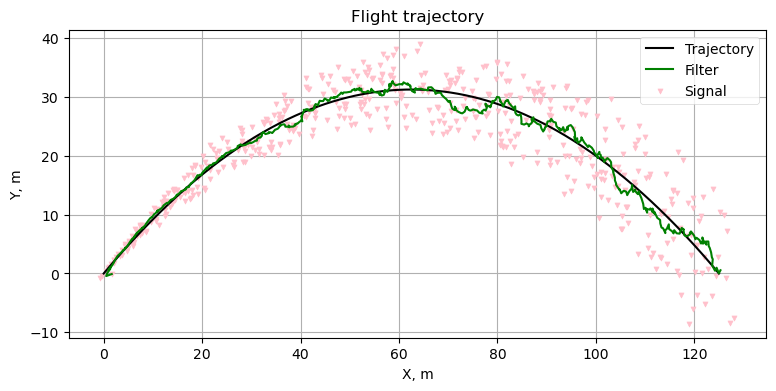
\includegraphics[width=0.9\textwidth]{images/kalmanfilter1.png}
\end{center}
\caption{Полёт тела в плоскости $XY$} \label{kalman1}
\end{figure}

Качественно из рис. \ref{kalman1} видно, что фильтр очень хорошо обрабатывает сигнал,  почти приближая его к истенному. Теперь выведем графики ошибок: \textit{показание сенсора - истинное значение} и \textit{фильтрованный сигнал - истинный}(рис.\ref{kalman2} и рис.\ref{kalman3}).

\begin{figure}[h!]
\begin{center}
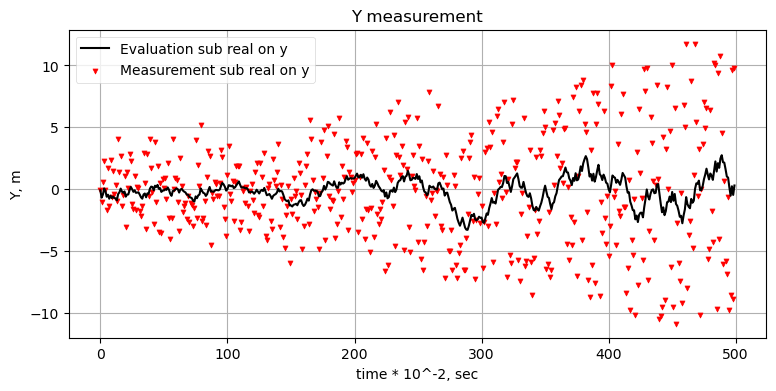
\includegraphics[width=0.9\textwidth]{images/kalmanfilter2.png}
\end{center}
\caption{Отклонение по $Y$} \label{kalman2}
\end{figure}

\begin{figure}[h!]
\begin{center}
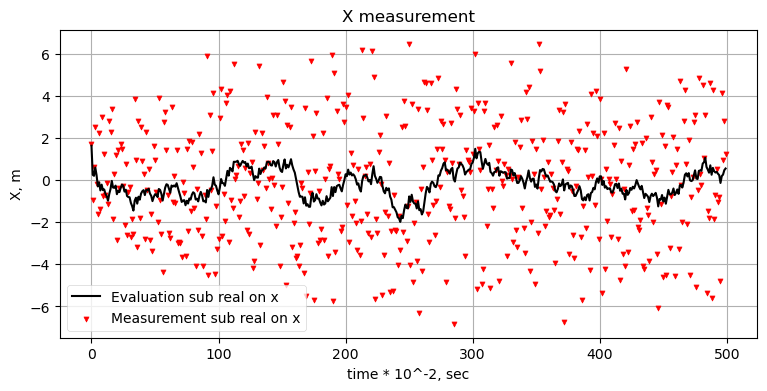
\includegraphics[width=0.9\textwidth]{images/kalmanfilter3.png}
\end{center}
\caption{Отклонение по $X$} \label{kalman3}
\end{figure}
По графикам можно численно убедиться, насколько точно мы воспроизводим действительный сигнал из  полученных измерений. Выведем также зависимости диагональных элементов в матрице ковариации $P$, соответствующих ошибкам по координатам $X$ (рис. \ref{kalman4}) и $Y$(рис. \ref{kalman5}):


\begin{figure}[h!]
\begin{center}
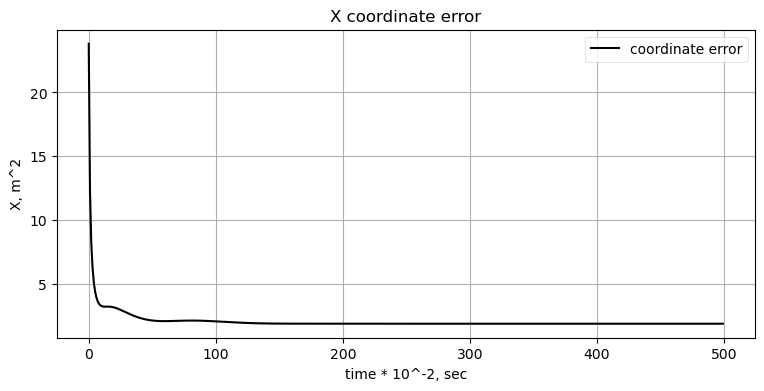
\includegraphics[width=0.9\textwidth]{images/kalmanfilter4.png}
\end{center}
\caption{Среднеквадратичная ошибка по $X$} \label{kalman4}
\end{figure}

\begin{figure}[h!]
\begin{center}
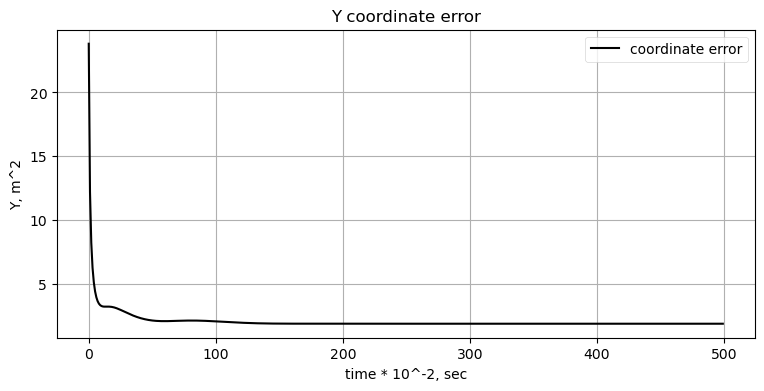
\includegraphics[width=0.9\textwidth]{images/kalmanfilter5.png}
\end{center}
\caption{Среднеквадратичная ошибка по $Y$} \label{kalman5}
\end{figure}

\newpage
Как видно из графиков \ref{kalman4} и \ref{kalman5}, ошибка падает,  т.е.  мы становимся более уверенными в конечном результате. Однако,  она не обращается в ноль,  а достигает своего постоянного значения.

\newpage
\subsection{Итог}
\begin{itemize}
\item Фильтр Калмана - это линейная модель;
\item Решается задача по минимизации среднеквадратичного отклонения;
\item Существует аналитическое решение по поиску весовых коэффициентов в матрице $K$;
\item Высокое приближение фильтрованного сигнала к истинному.
\end{itemize}

\newpage
\section{Рекуррентные нейронные сети}
Перед обсуждением структуры рекуррентных нейронных сетей,  далее именнуемых RNN\footnote{RNN (англ.  recurrent neural network) -  рекуррентная нейронная сеть.}, рассмотрим более простые архитектуры и  другие важные понятия,  необходимые в RNN. 

Основой любой NN\footnote{NN (англ.  neural network) -  нейронная  сеть.} является линейная модель.

\subsection{Линейные модели}

Линейная модель - это базисная конструкция,  которая по набору признаков  принимает решение об принадлежности или свойствах объекта,  которому они принадлежат.

$$Y=X_1+X_2+X_3,$$
$Y$ -  решение  системы,  $X_i$ - категориальные признаки\footnote{Многие методы предполагают, что все признаки $X\in R$. Однако, в некоторых задачах признаки могут принимать значения из множеств, не совпадающих с множествами вещественных чисел. Такие признаки называются категориальными, факторными или номинальными $^\text{\cite{nnkategor}}$.}.

 Линейная модель решает задачи:
\begin{itemize}
\item Классификации - формализованная задача, в которой имеется множество объектов (ситуаций), разделённых некоторым образом на классы. Задано конечное множество объектов, для которых известно к каким классам они относятся. Это множество называется выборкой. Классовая принадлежность остальных объектов неизвестна. Требуется построить алгоритм, способный классифицировать произвольный объект из исходного множества (работа с дискретными величинами).
\item Регрессии - формализованная задача, в которой есть множество объектов, есть функция на нем. Для некоторого подмножества объектов задано значение функции. Нужно научиться предсказывать значение функции на других объектах. Качество выполнения задачи определяется функционалом качества. Например, MSE (работа с непрерывными величинами).
\end{itemize}

Подробнее о постановках задач классификации, регрессии и других задач в курсе лекций К. В. Воронцова\cite{voron}.  Мы же рассмотрим задачу линейной регрессии: 

$$\mathds{E}(Y|X)=f(X);$$

или

$$Y=f(X)=\varepsilon;$$

$f$ - функция регрессии, и для линейной модели имеет вид:

$$f_\omega(x)=\omega_0+\sum\limits_{i=1}^p\omega_ix_i\equiv x^T\omega;$$

где $\omega=(\omega_0,\omega_1,...,\omega_n)^T$ - веса, $x=(1,x_1,...,x_n)^T$- признаки объектов. 

Пусть теперь мы имеем  $n$ объектов: $(x^i,y^i)$ $i=\overline{1,n}$,  где $y^i\in R$ - метки  объекта,   $x^i\in R$ - описание  объекта.

Тогда матрицы  наших  объектов: $$X=[x^1,...,x^n]^T, X\in  R^{n\times p};\qquad Y=[y^1,...,y^n]^T, Y\in  R^{n}.$$

 \begin{equation}\label{Xw}
f_\omega(X)=X\omega=\widehat{Y};
\end{equation}
 
 Осталось только выбрать веса для  матрицы $\omega$. Введём функцию эмпирической ошибки,  как сумму всех наших потерь:
 
 $$\text{Empirical risk}=\sum\limits_\text{by objects}\text{Loss on object}.$$
 
И будем её минимизировать по весам $\omega$,  то есть:

$$Q(X)=\sum\limits_{i=1}^{n}L(y^i,f_\omega(x^i))\longrightarrow\min$$

 Таким образом мы сможем,  подбирать $\omega$. 
 
 В общей сложности для разных задач  существуют разные функции потерь. В данной работе (в задачи регрессии) будет использоваться функция среднеквадратичного  отклонения:
 \begin{equation}\label{MSE}
\text{MSE loss: } L(y_t,y_p)=(y_t-y_p)^2.
\end{equation}
 
Тогда:

$$Q_\text{MSE}=(Y-X\omega)^T(Y-X\omega)\longrightarrow\min;$$

Для минимизации исследуем функцию потерь,  взяв производную:

$$\nabla_\omega Q_\text{MSE}=-2Y^TX+2X^TX\omega^T=0.$$

Откуда матрица весов:
\begin{equation}\label{w}
\omega^*=(X^TX)^{-1}X^TY;
\end{equation}

По  Теорема Гаусса — Маркова$^\text{\cite{voron}}$,  данная матрица единственна.  В данной постановке задачи и в выводе её решения,  чётко прослеживается аналогия с линейной  моделью фильтра  Калмана,  откуда можно сделать вывод, что фильтр Калмана - это модель  задачи линейной  регрессии.

Как видно из формулы \ref{w}, решение $\omega^*$ не устойчиво, так как матрица  $X^TX$ не всегда имеет обратную.  Тут следует  дополнить  задачу и  потребовать  от неё усточивости  в решении - провести  регуляризацию.  Добавим к нашей функции  ошибки вторую  норму матрицы  весов, умноженную на квадрат коэффициента $\lambda$:

$$L_2=||Y-X\omega||^2_2+\lambda^2||\omega||^2_2$$ 
$$\omega^*=(X^TX+\lambda^2I)^{-1}X^TY;$$

 Данный метод регуляризации (сдвиг решения) называется $L_2$ регуляризацией или регуляризацией Тихонова$^\text{\cite{Spokbook}}$.  Существует также $L_1$  регуляризация - регуляризация через манхэттенское расстояние$^\text{\cite{lasso}}$.  
 
Описанное выше аналитическое решение включает в себя инверсию матрицы $X^T X$ (или $X^T X + \lambda I$), что довольно дорого с точки зрения вычислительных ресурсов. Сложность инверсии матрицы можно оценить как $O (p^3 + p^2 N)$. Это приводит нас к итеративным методам оптимизации, которые являются более эффективными и фактически являются основным подходом к оптимизации в машинном обучении.

Градиентный спуск - один из самых популярных методов оптимизации. Стоит отметить тот факт, что цель минимизации (максимизации) (например, значение функции потерь) должна быть дифференцируема по параметрам модели.  Используя градиентный спуск, вектор весов $\mathbf{w}^{(t+1)}$ на шаге $t+1$ можно выразить в следующем виде:

$$
\mathbf{w}^{(t+1)} = \mathbf{w}^{(t)} - \eta_t \nabla Q(\mathbf{w}^{(t)}),
$$
где $\eta_t$ шаг градиента (называемый \textit{learning rate}(англ.)).

Градиент в случае функции потерь MSE принимает следующий вид:

$$
\nabla Q(\mathbf{w}) = -2X^TY + 2X^TX\mathbf{w} = 2X^T(X\mathbf{w} - Y).
$$

В этом случае сложность составляет всего $O (pN)$. Чтобы сделать его еще более эффективным,  мы будем использовать стохастический градиентный спуск,  который вычисляет градиент только по некоторому случайному подмножеству данных(англ. batch) $K$ точек, так что конечная сложность уменьшается до $O(pK)$, где $K << N$.

Данный процесс,  когда градиентным спуском нашей функии ошибки подбирается матрица весов  $\omega$,  назывется обучением (англ.training).

\subsection{Функции активации}
Линейные модели отлично себя проявляют в классификации или  в регрессии  \textbf{линейных} данных,  показывают также достойные  результаты  с данными,  которые неплохо аппроксимируются прямой.  Например, малый участок зашумленной траектории,  обрабатываемый фильтром Калмана. 

Однако, большенство данных (траетория движения), плохо или вообще не аппроксимируются прямой, так как имеют другие  зависимостии(например логарифмические),  поэтому нам необходимо <<уйти>>  от \textit{нелинейного} признакового пространства в новое пространство(чаще всего  линейное), где мы сможем работать  с  новыми  признаками  знакомыми способами.  Идея  очень проста,  добавим \textbf{нелинейное преобразование}:

\begin{enumerate}
\item Входные данные: $X$;
\item Линейная модель: $h=X\omega$;
\item Нелинейное преобразвание: $\sigma(h)$;
\item MSE;
\item Предсказание.
\end{enumerate}

Нелинейноую функцию, в частности $\sigma$,  называют \textbf{функцией  активации}. Функций активаций бывает множество  видов,  приведем в  качестве примера пару из них:

\begin{itemize}

\item $\sigma(x)=\frac{1}{1+e^{-x}},$ $R\longrightarrow(0,1)$;

\item $\th(x)$,  $R\longrightarrow(-1,1)$;

\item $\ln(1+e^x)$,  $R\longrightarrow(0,\infty)$;

\end{itemize}

Функции активации  позволяют  нашей сети,  переводить признаки  в новое  удобное для себя  пространство,  где NN сможет с ними работать или перевести в еще одно признаковое пространство.  Множество таких линейных и  нелинейных преобразований называются  слоями.  Присутсвие функций активации в преобразованиях NN является одной из отличительных черт,  почему NN превосходит классические линейных модели в работ с нелинейными данными.

Для работы NN обычно имеет в каждом слое(преобразовние) обучаемый парметр или несколько, а также требует, чтобы все слои имели производную в точке, для возможности  обучаться градиентным  спуском.

\textbf{Примечание.}

Название и происхождение функций активации уходит в биологию и психологию.  Когда люди решили смоделированть поведение  \textit{нейронов},  они обнаружили, что множество  нейронов передают  потенциал одному,  и тот, после превышения порогового значения(\textit{активации}),  начинает передавать накопившийся потенциал остальным.  То есть для работы модели нейронов  или нейронной сети требуется функция  активации,  которая была бы  <<дифференцируема>>.  Первой такой функцией стала  $\sigma$.

\subsection{RNN}
Чаще всего данные,  которые нам встречаются, и которые необходимо обрабатывать,  обладают структурностью.  Например, речь,  где порядок слов и букв обладает собственной архитектурой и несёт важную информационную нагрузку.  При обработке тут важно учитывать свойства структурности информации.  

Траектория движения имеет последовательность точек,  которые привязаны ко времени,  это означает,  что каждая последующая координата зависит от совокупности предыдущих.  То есть при фильтрации новых значений мы помимо знаний о физической природе объекта можем пользоваться доступным контекстом - уже обработанными точками траектории. 

\subsubsection{Простейшая схема  RNN}

\begin{figure}[h!]
\begin{center}
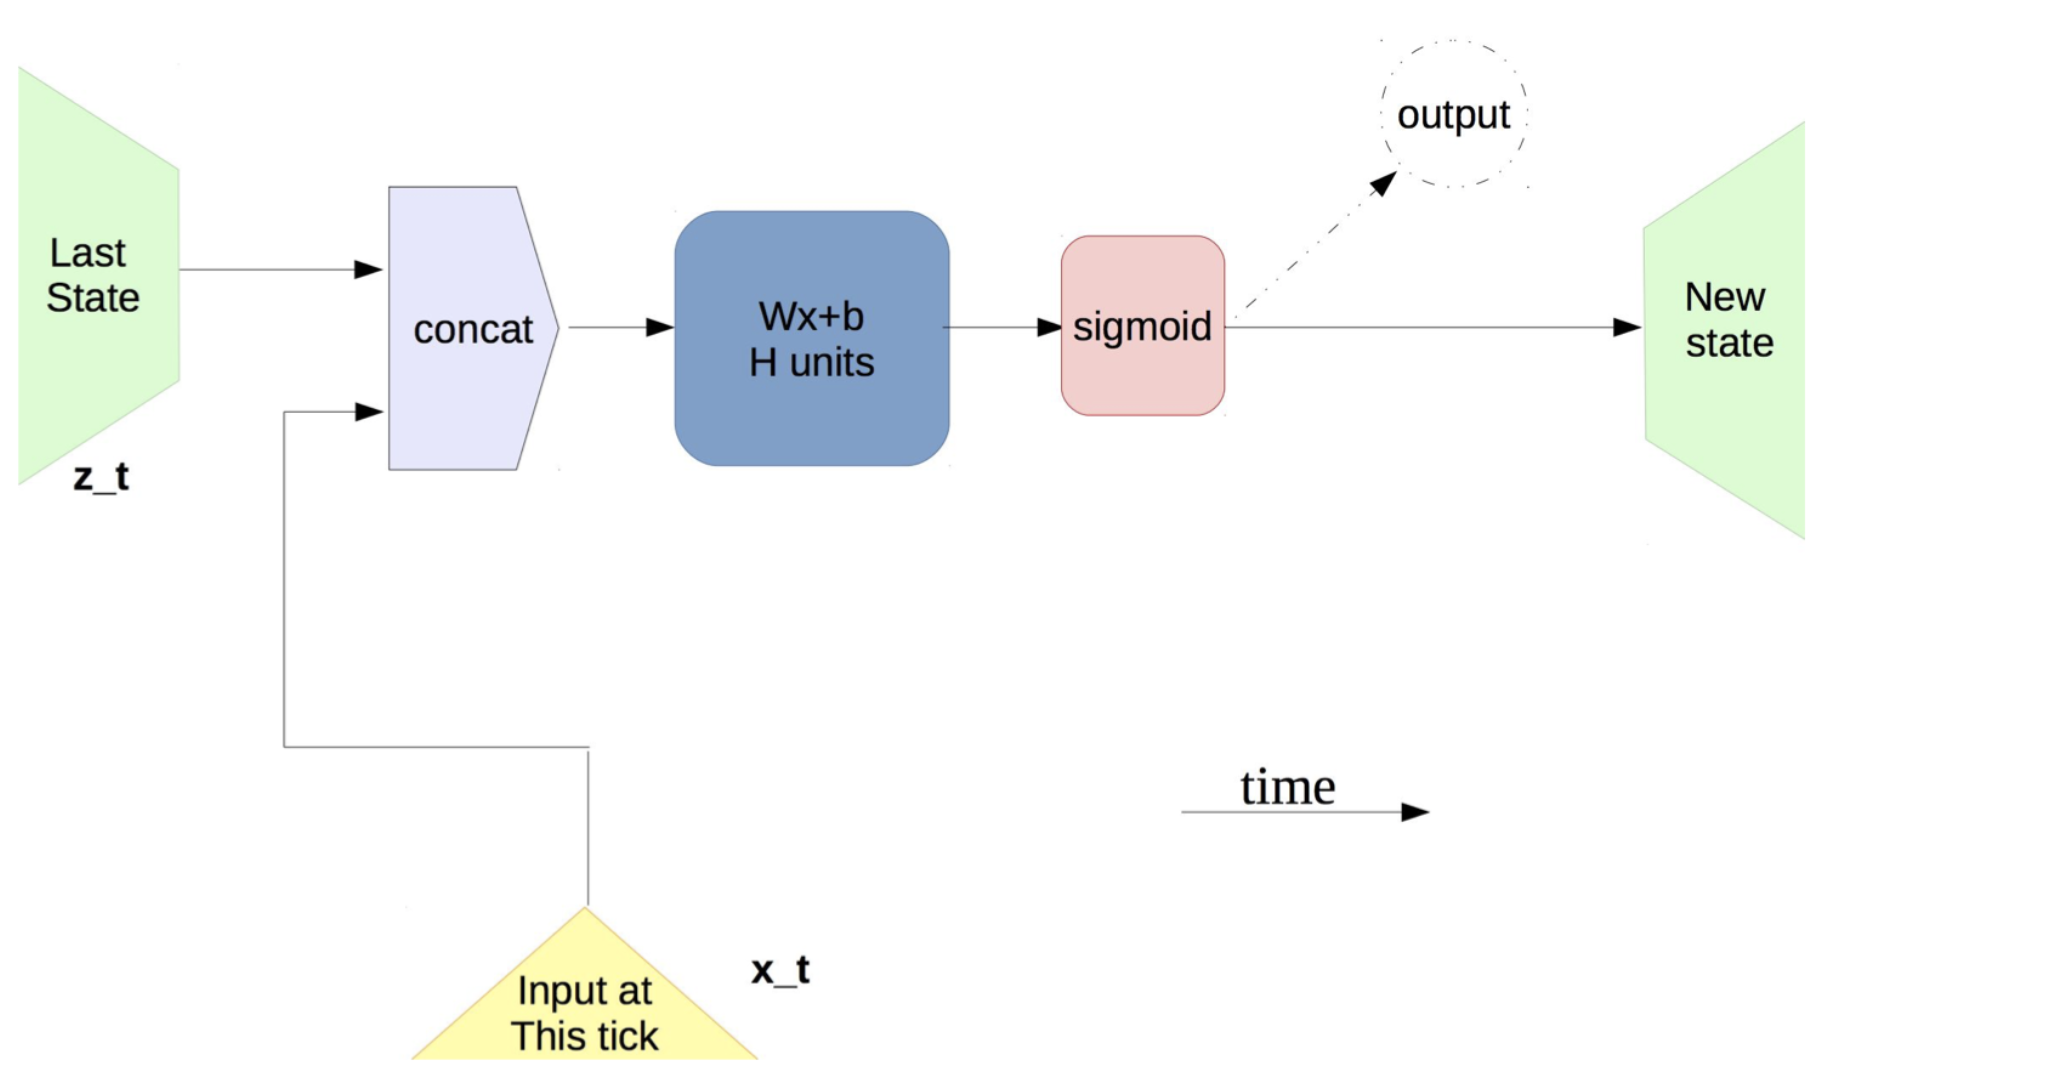
\includegraphics[width=0.9\textwidth]{images/RNN1}
\end{center}
\caption{Схема RNN loop$^\text{\cite{NN}}$.} \label{RNN1}
\end{figure}

Пусть у нас уже имеются данные и часть контестка,  связанного с ними. Теперь мы хотим <<обогатить>> контекст следующими данными,  и получить результат обработанных значений в совокукпности с предыдущими.  Для этого мы можем предствить свои данные в виде векторов:  $C$ - контекст фиксированной размерности,  $i$  -  входные данные фиксированной размерности.  Для объеденения старой и полученной инфомации можно конкатенировать вектора  $C$ и $i$ в $[C,i]$.  Для получения новых данных(нужной размерности) можно провести линейное преобразоввание: $W\cdot[C,i]+b$.  Так как мы хотим построить  NN,  она должна иметь  нелинейность в своих преобразованиях, поэтому добавим функцию активации после линейного слоя: $\sigma(W\cdot[C,i]+b)$.  Мы получили композицию преобразований, способную называться нейронной сетью, так как у нас есть нелинейность в преобразованиях,  веса $W$ для обучения.  Скажем, что  $W\cdot[C,i]+b$ порождает вектор размерности, соответсствующей изначальному контексту $C$,   следовательно, мы получили обновленный контекст,  способный участвовать в дальнейшей циклической обработке данных.  Нейронные сети данного типа,  называют рекурентными,  а один оборот процесса - петлёй (англ.  loop), рис.  \ref{RNN1}.

\begin{figure}[h!]
\begin{center}
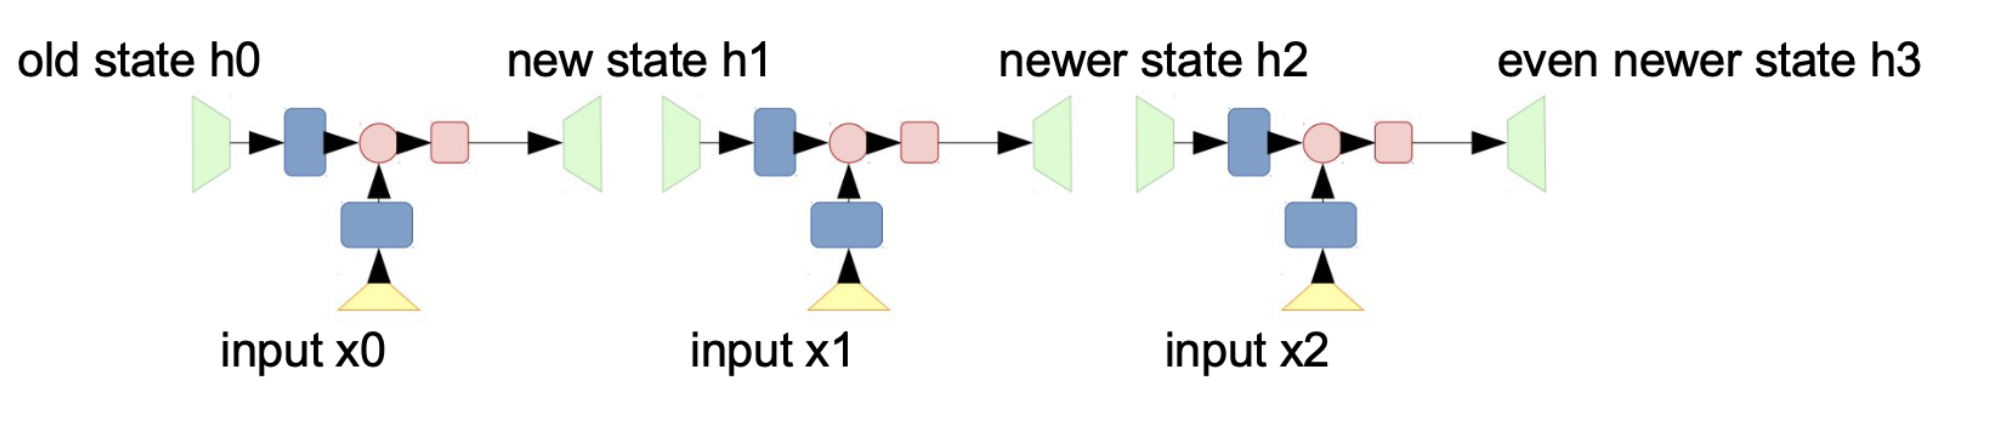
\includegraphics[width=1\textwidth]{images/RNN2}
\end{center}
\caption{Простейшая схема RNN$^\text{\cite{NN}}$.} \label{RNN2}
\end{figure}

На  рис. \ref{RNN2} показана схема циклической работы RNN.

Можно заметить, что первоначальная информация вектора контекста после нескольких циклов добавления новых данных быстро <<забывается>> из-за фиксированной размерности $C$, и мы теряем картину начальных событий.  Учитывая, что в данных может присутвовать много зашумленных или ненужных значений,  имеет смысл запоминать важную информацию и пропускать остальную - дать нашей сети  возможность выбирать что нужно запомнить, а что  нет.

\newpage
\subsubsection{Фильтр Калмана и LSTM}

LSTM (англ.  Long Short-Term Memory) - рекуррентная нейронная сеть, с кратковременной и долговременной памятью\footnote{Основной материал по LSTM можно найти в лекции Стэнфорда \cite{RNN}}.  Основная структура схемы LSTM на  рис.  \ref{RNN3}.

\begin{figure}[h!]
\begin{center}
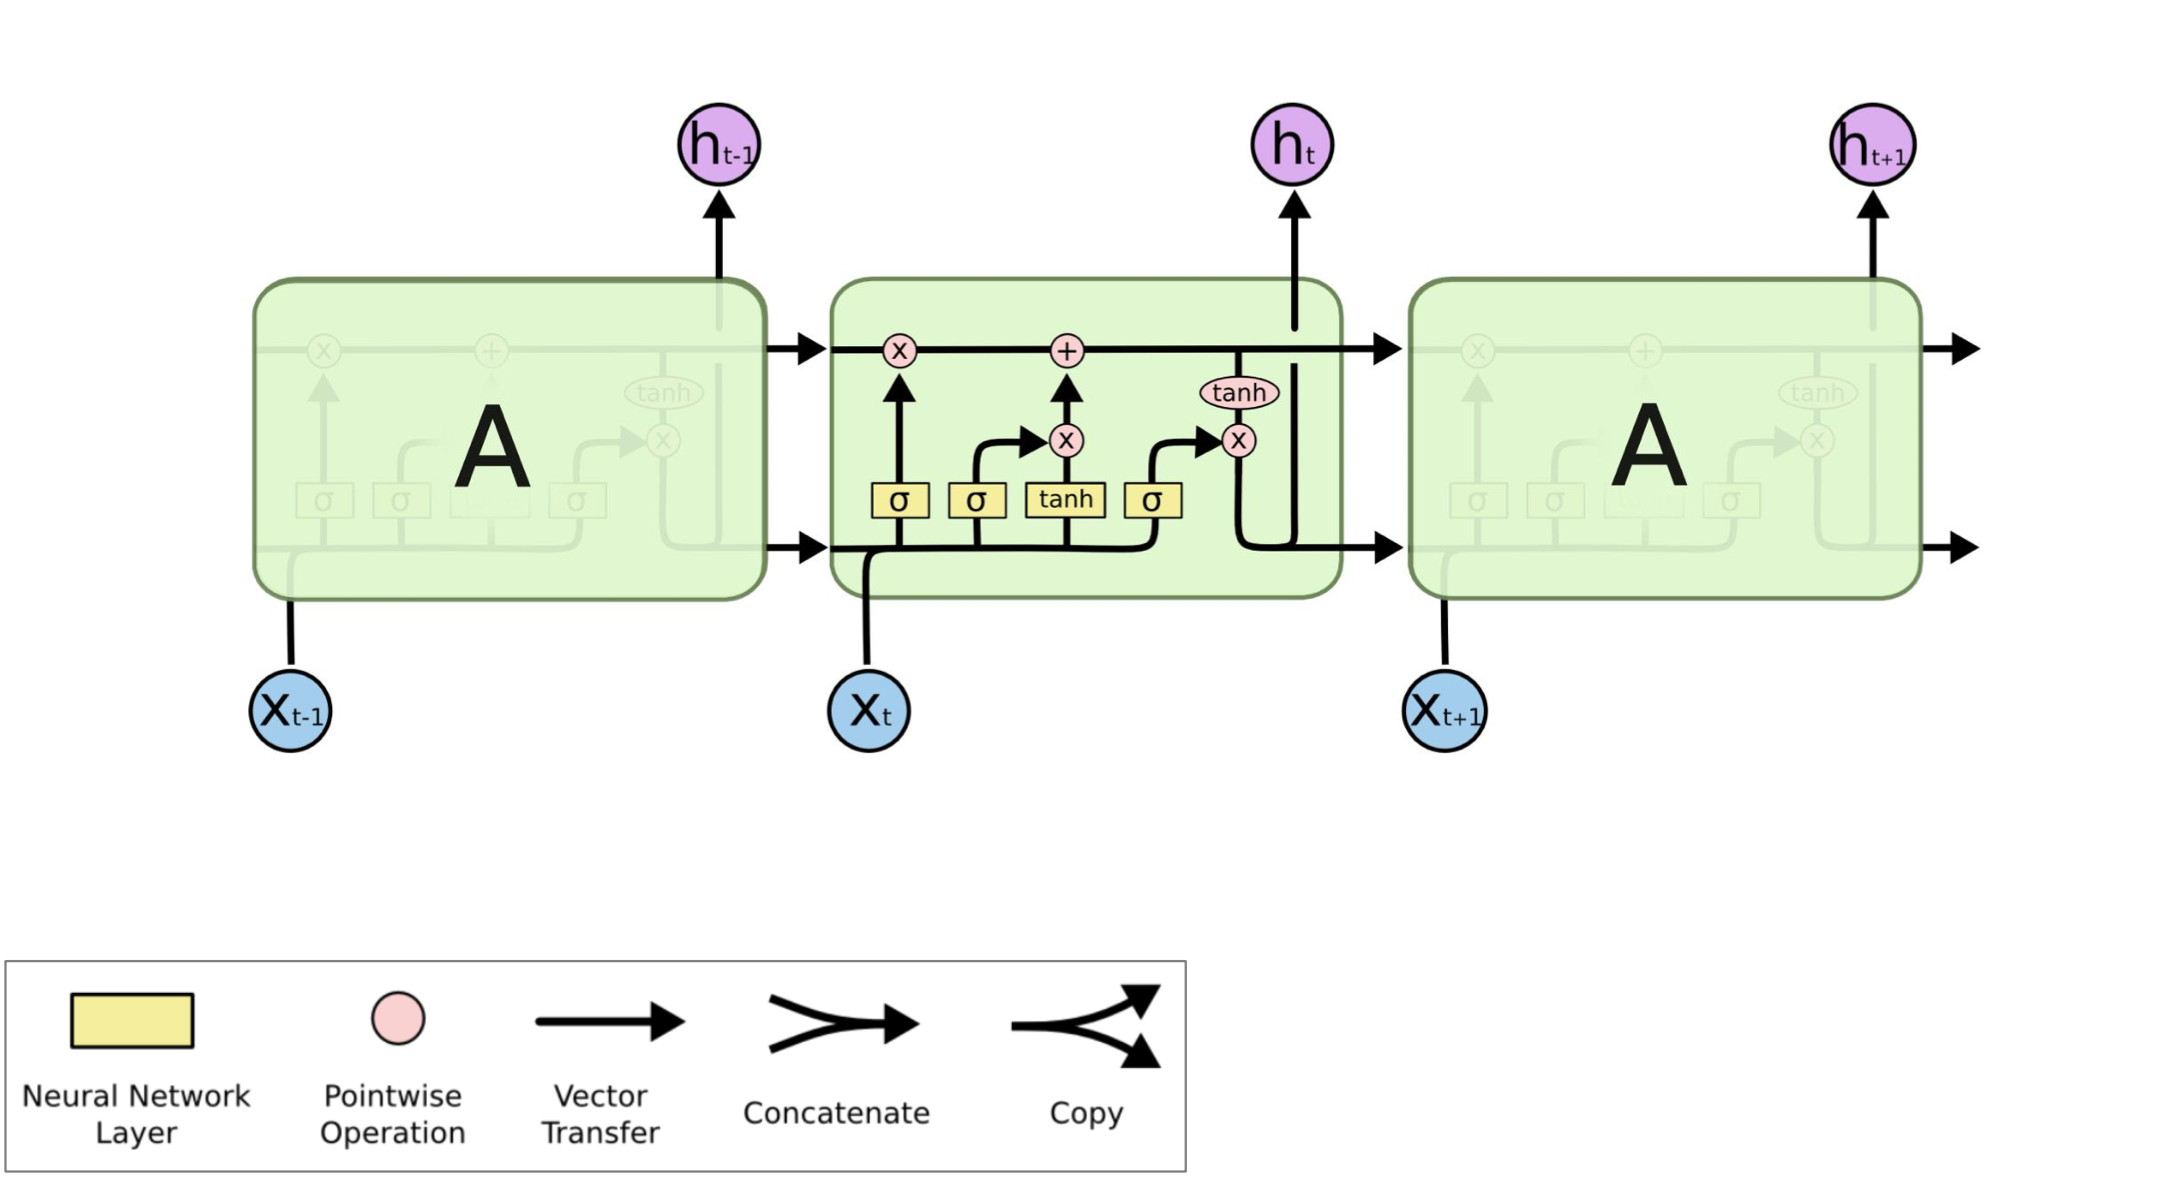
\includegraphics[width=1\textwidth]{images/RNN3}
\end{center}
\caption{LSTM$^\text{\cite{RNN}}$.} \label{RNN3}
\end{figure}
В схеме используется функция активации $\tanh$,  позволяющая держать распределение наших данных в интервале $(-1,1)$,  а также центрировать их относительно $0$,  поэтому $\tanh$ не перегрузится от больших значений, а градиент не взорвется.\footnote{Взрыв градиента - понятие, когда градиент быстро растёт и вызывать переполнение данных.} 

\begin{figure}[h!]
\begin{center}
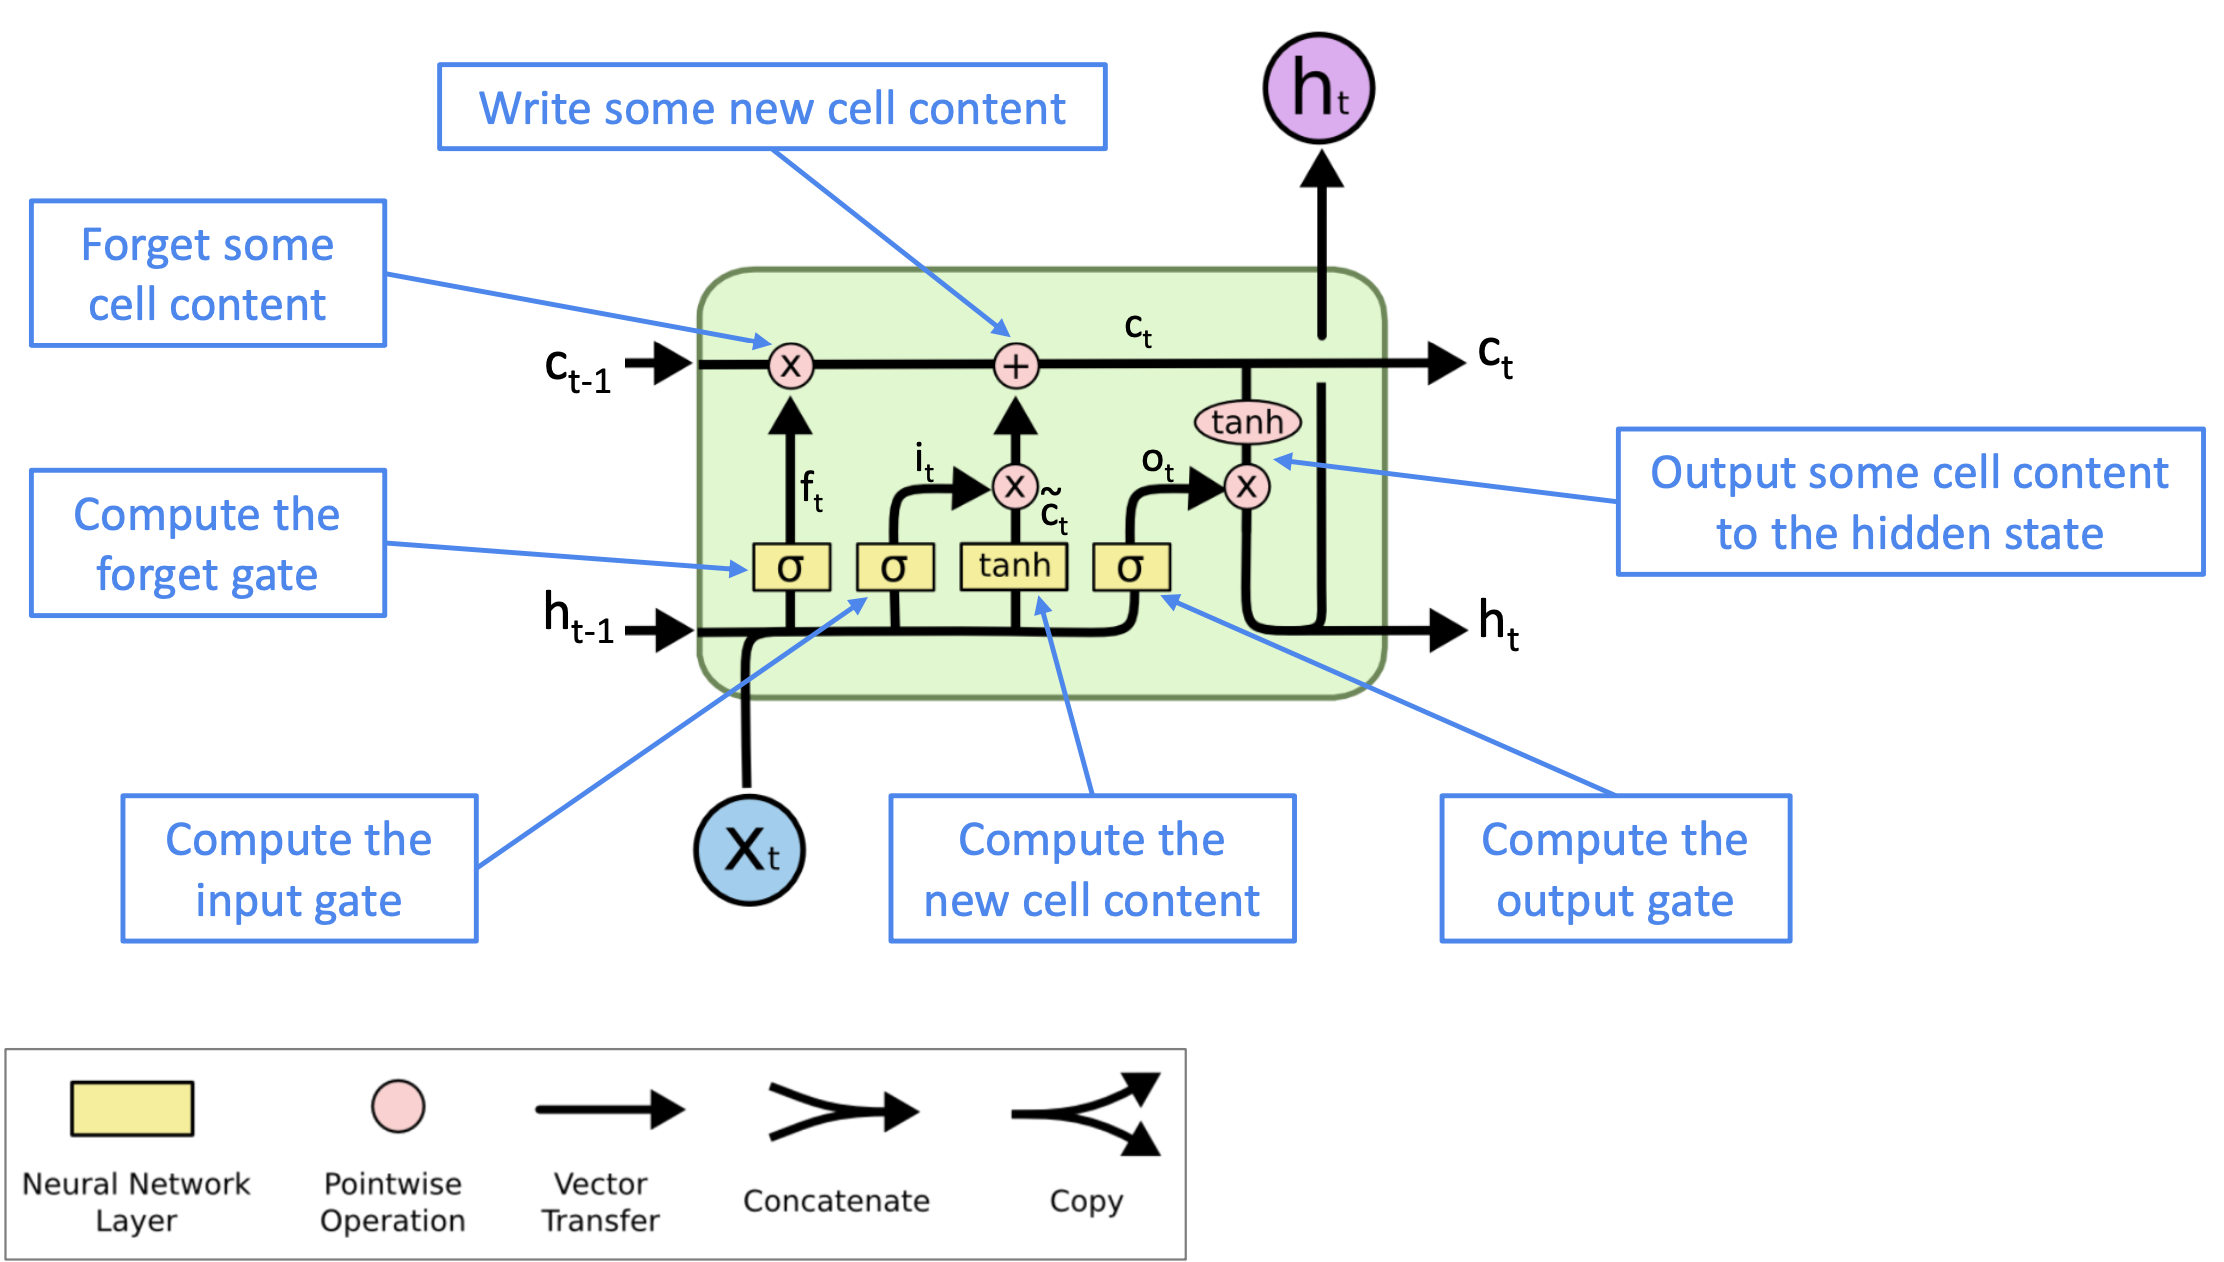
\includegraphics[width=1\textwidth]{images/RNN4}
\end{center}
\caption{LSTM loop$^\text{\cite{RNN}}$.} \label{RNN4}
\end{figure}

LSTM использует два вектора контекста: $С$  - долговременная память, $h$ - кротковременная память.  Задача выбора: какую информацию оставить, а какую забыть,  является бинарной классификацией. $f_t$ - вектор "забывания" содержит $0$ в своих местах,  где  данные нужно стереть,  и  $1$,   где сохранить:

$$f_t=\sigma(W_f\cdot[h_{t-1},x_t]+b_f).$$

Функция  $\sigma$ бинарно классифицирует данные $(0,1)$ , после чего совершается поэлементное умножение $f_t$ на  $C_{t-1}$. Теперь нужно запомнить навую информацию для этого, снова решаем задачу классификации, пусть $i_t$ - вектор "запоминания" аналогичный $f_t$:

$$i_t=\sigma(W_i\cdot[h_{t-1},x_t]+b_i).$$

А также нам нужны сами данные $\widetilde{C}_t$ для запоминания:

$$\widetilde{C}_t = \tanh(W_C\cdot[h_{t-1},x_t]+b_C).$$

Обновление долговрменной памяти:

$$C_t=f_t\cdot C_{t-1}+i_t\cdot \widetilde{C}_t.$$

Изменение  краткосрочной памяти,  аналогично $C_t$:

$$o_t=\sigma(W_o\cdot[h_{t-1},x_t]+b_o);$$

$$h_t=o_t\cdot\tanh(C_t).$$
 
 Для решения задачи фильтрации в алгоритме Калмана заменим пункт \textbf{Обновления}  формулы \ref{K}, \ref{KP} на LSTM.  Сеть  будет получать зашумленный сигнал $x_{\text{noise}_t}$, выводить уже отфильтрованное значение $h_t$. Далее по формулам \ref{xFuB} на основее предыдущего значения фильтрации,  пользуясь свойствами физической модели объекта, предсказываем предположетельное значение $\widetilde{x}_t$.  Конкатенируем $[\widetilde{x}_t,h_t]$ и совершаем линейное преобразование,  получая вектор  размерности  координат точки:
 
$$\widetilde{x}_t =Fx_{t-1};$$

\begin{equation}\label{KRNN}
x_t=W_K\cdot[\widetilde{x}_t,h_t]+b_k.
\end{equation}


\begin{figure}[h!]
\begin{center}
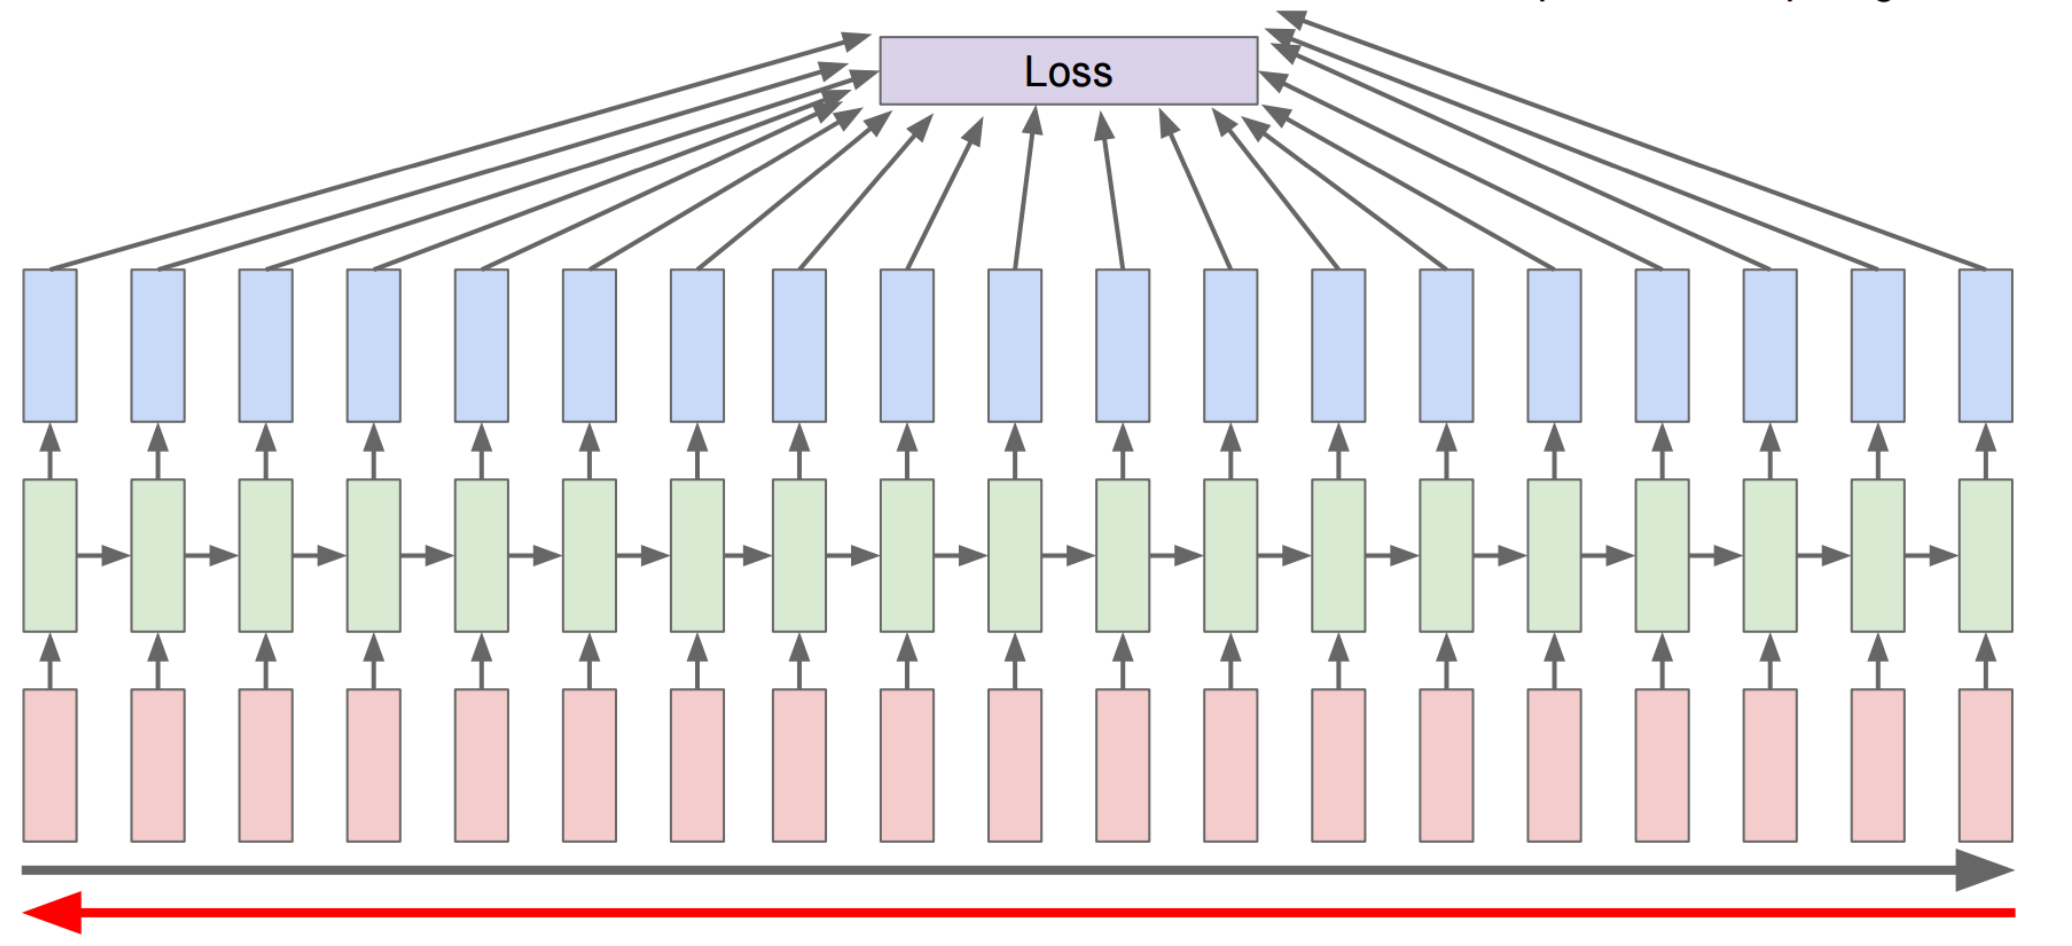
\includegraphics[width=1\textwidth]{images/RNN5}
\end{center}
\caption{Обучение во времени.} \label{RNN5}
\end{figure}

Последний линейный слой (формула \ref{KRNN}),  описанный выше, также будет обучаться нейронной сетью, так как является её частью. Подбирать весовые параметры NN будем методом стахостического градиентного спуска от Loss функции \ref{MSE}(фильтрация сигнала - задача регрессии),считая производные слоев$^\text{\cite{mtrixgrad}}$ рис.  \ref{RNN5}.

Практическую реализацию модели на Python можно смотреть в \hyperref[appendix]{Приложении}.
\newpage
\section{Реализация}

Основной код программы, на который мы будем ссылаться,  приложен  в конце отчёта(\hyperref[appendix]{Приложение}). Необходимые минимальные выдержки из оригинала будут дополнительно цитироваться.

\subsection{Обзор}

Архитектура сети уже обсуждалась в разделе \hyperref[RNNfilter]{Фильтр Калмана и LSTM}. Рассмотрим в общем плане практическую реализацию.  Нейронная сеть написанна на основе фреймворка машинного обучения PyTorch с открытым исходным кодом. Вначале процесса данные предобрабатываются для обучения:
\begin{lstlisting}
class TrajectoryDataset() 
def create_dataset()
\end{lstlisting}

Создаем класс данных(основанный на стандартах Dataset PyTorch), предварительно  приводя его в стандартизированный вид фиксированной длинны, создаем зашумленные сигналы.

\begin{lstlisting}
class ModuleRNN(nn.Module)
\end{lstlisting}
Класс нейронной сети, который содержит в себе главную архитиктуру системы. В методе forward описан алгоритм, обсужденный в главе \hyperref[RNNfilter]{Фильтр Калмана и LSTM}:

\begin{lstlisting}[label=some-code,caption=ModuleRNN.forward(), language=Python]
def forward(self, new_data, flash_memory, short_term_memory, long_term_memory, F):

        memory = torch.cat([new_data, short_term_memory], dim=-1)

        forgetfulness = torch.sigmoid(self.rnn_forget(memory)) #forgetting dataforgetting data
        conservation = torch.tanh(self.rnn_save(memory)) #the acquisition of new data
        information = torch.sigmoid(self.rnn_data_selection(memory))

        long_term_memory = (forgetfulness * long_term_memory) + (information * conservation)

        short_term_memory = torch.sigmoid(self.rnn_quick_overview(memory)) * torch.tanh(long_term_memory)
        
        with torch.no_grad():
            flash_memory = self.predict_Kalman(F, flash_memory)
            flash_memory_grad = flash_memory[:,0::3]


        predicted_data = self.rnn_prediction(torch.cat([flash_memory_grad, short_term_memory], dim=-1))

        with torch.no_grad(): 
            flash_memory[:,0::3] = predicted_data

        return predicted_data, flash_memory, short_term_memory, long_term_memory
\end{lstlisting}

В коде имеются области with torch.no\_grad(), отключающие поиск производных для вошедших в них операций, так как они не являются дифференцируемыми\footnote{Cрезы тензоров используются для оптимизации, так как являются более быстрыми и эффективными операциями чем  матричные умножения}.

\begin{lstlisting}
def rnn_loop()
\end{lstlisting}

Главный цикл в котором работает RNN.

\begin{lstlisting}
def traning_fun()
\end{lstlisting}

Основаня функция, в которой тренируется и проходит валидацию нейронная сеть.

\begin{lstlisting}
def testing_fun()
\end{lstlisting}

Функция тестирования NN.

\begin{lstlisting}
def save_checkpoint()
def load_checkpoint()
\end{lstlisting}

 Также присутствуют функции,  сохраняющие и загружающие (обученную) нейронную сеть. \textbf{Важно:}  NN  будет работать только с изночальной моделью класса \textbf{ModuleRNN}(сохраняйте архитектуру ModuleRNN).
 
\subsection{Обучение и валидация}\label{trainval}

Приведём процесс  обечения и  валидации\footnote{Валидация - это проверка данных на соответствие заданным условиям и ограничениям.} в виде графиков  зависимостей  от эпох\footnote{Эпоха - время, за которое обрабатываются все данные.}:
\begin{figure}[h]
\begin{minipage}[h]{0.49\linewidth}
\center{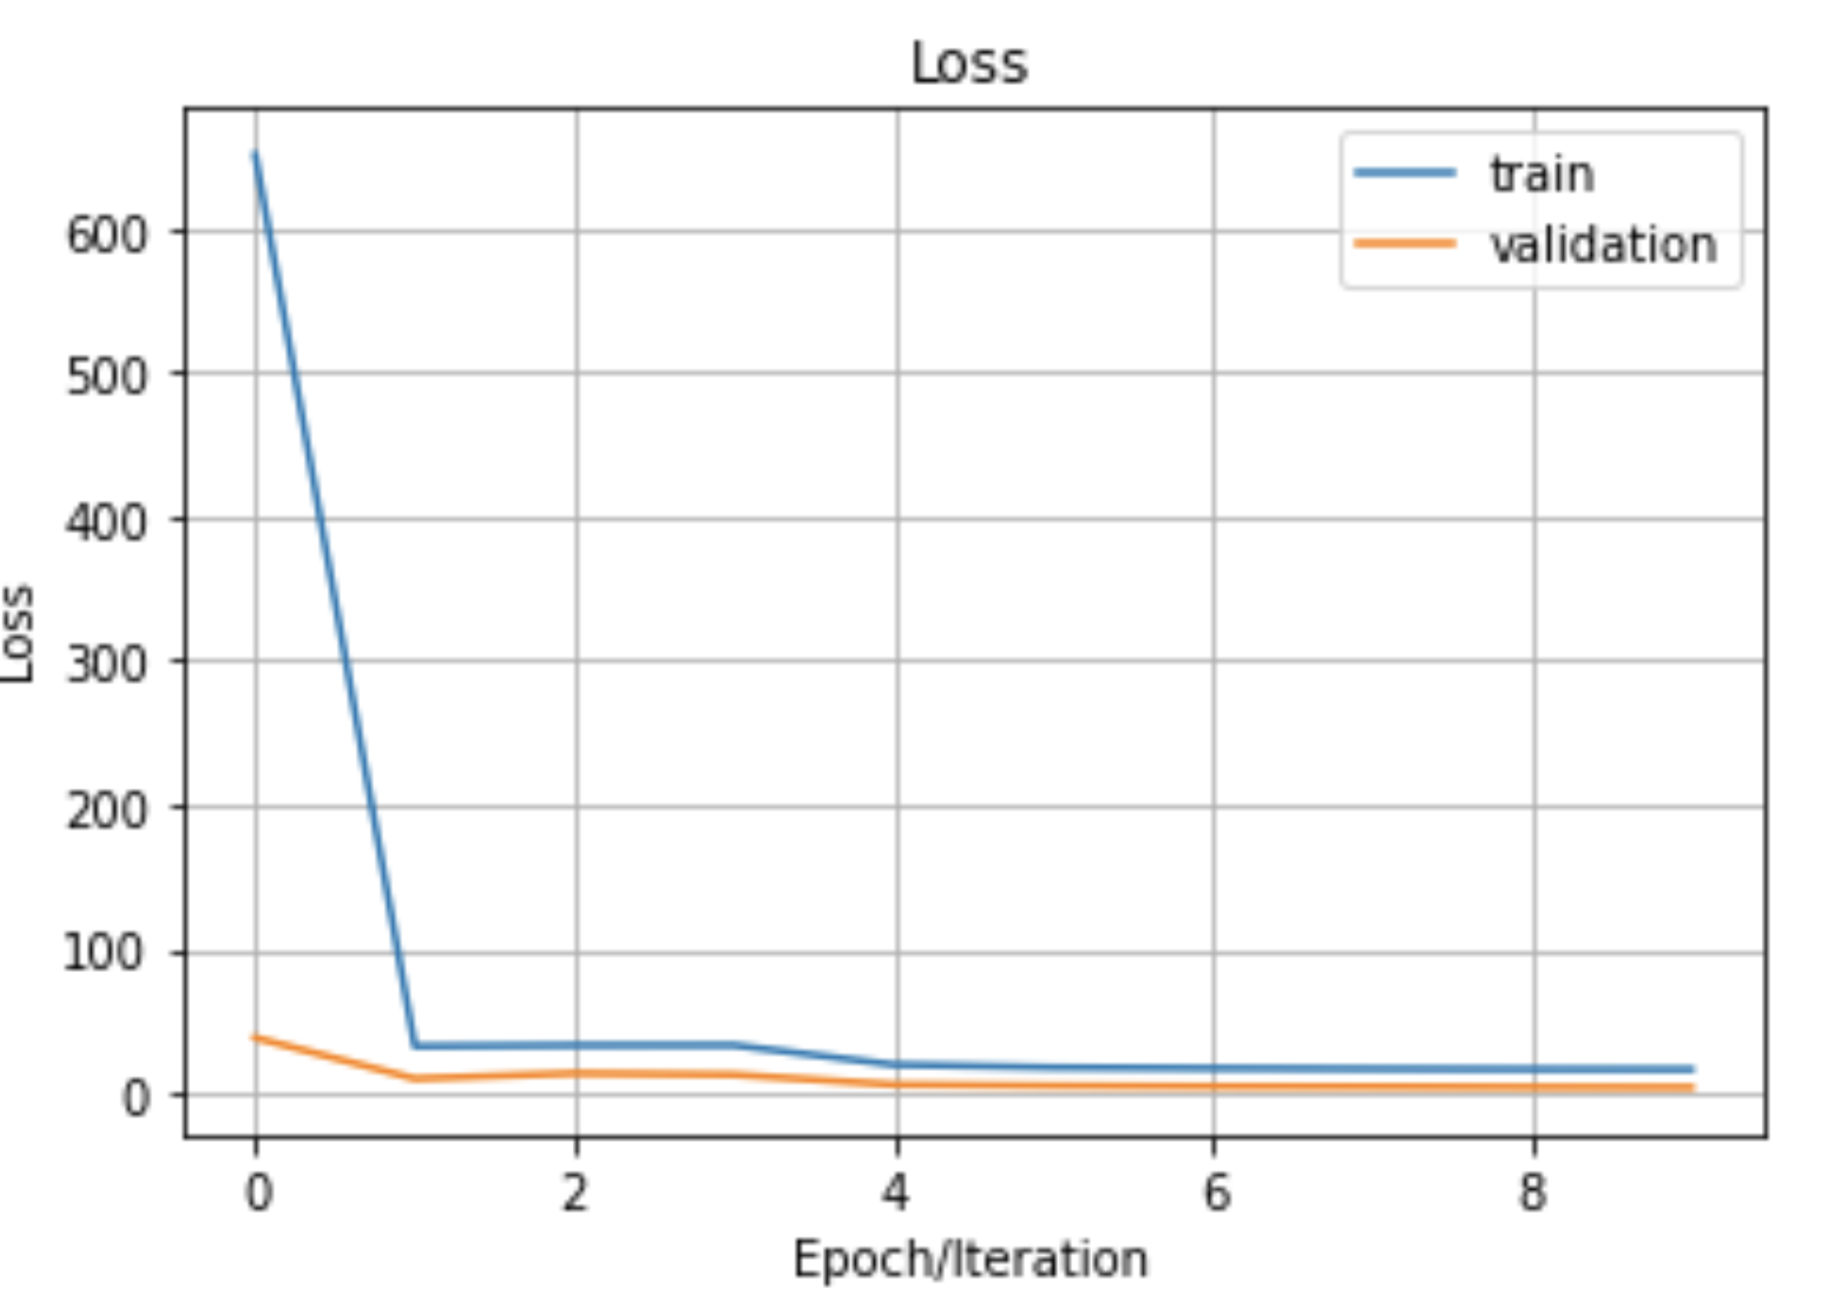
\includegraphics[width=1\linewidth]{images/losstrain.png} \\ а)}
\end{minipage}
\hfill
\begin{minipage}[h]{0.49\linewidth}
\center{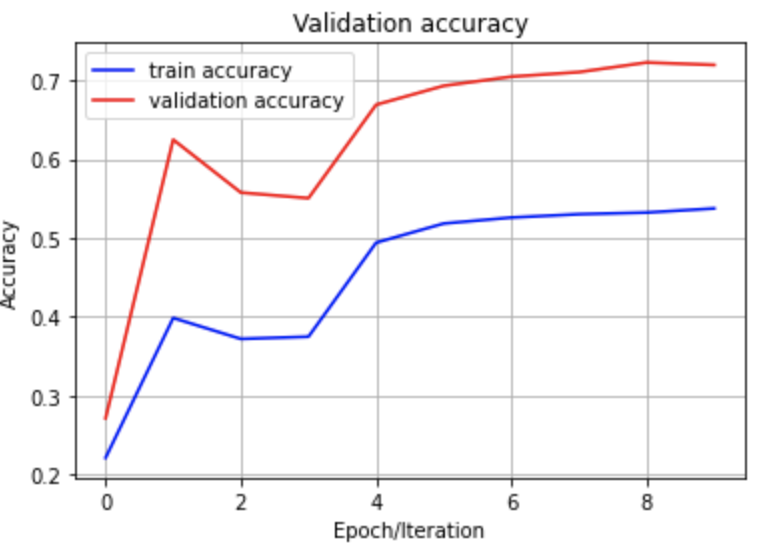
\includegraphics[width=1\linewidth]{images/valtrain.png} \\ б)}
\end{minipage}
\caption{Процесс обучения и валидации. а) график зависимости средней по данным MSE ошибки от эпохи; б) график зависимости средней по данным точности от эпохи.}
\label{train}
\end{figure}

Напомним, что подбираем веса парметров NN методом стохастического градиентного спуска от функции потерь MSE \footnote{MSE - функция потерь (англ. loss), cреднеквадратическая ошибка.}(формула \ref{MSE}):
$$\text{MSE loss: } L(y_t,y_p)=(y_t-y_p)^2.$$

"Точность" осуществляем подсчетом количества точек фильтрованного сигнала, отклонившихся  от оригинала не  более чем на $5\%$.

\begin{lstlisting}
def accuracy(x_pred, x_real, Discrepancy):
    delta = np.absolute(x_pred)-np.absolute(x_real)
    return np.sum(
        (np.absolute(delta/x_pred) <= Discrepancy)|
        (np.absolute(delta/x_real) <= Discrepancy))/ x_real.size
\end{lstlisting}

\textbf{Вывод:} Из падения графиков на MSE и росте на Accuracy видно,  что сеть обучается. Точность на валидации чуть выше $70\%$, это связано с регуляризацией\footnote{В данном случае говорится об  регуляризацие Dropout.} модели.

\subsection{Тестирование}
Приведём процесс тестирования в виде графиков:
 \begin{figure}[h]
\begin{minipage}[h]{0.49\linewidth}
\center{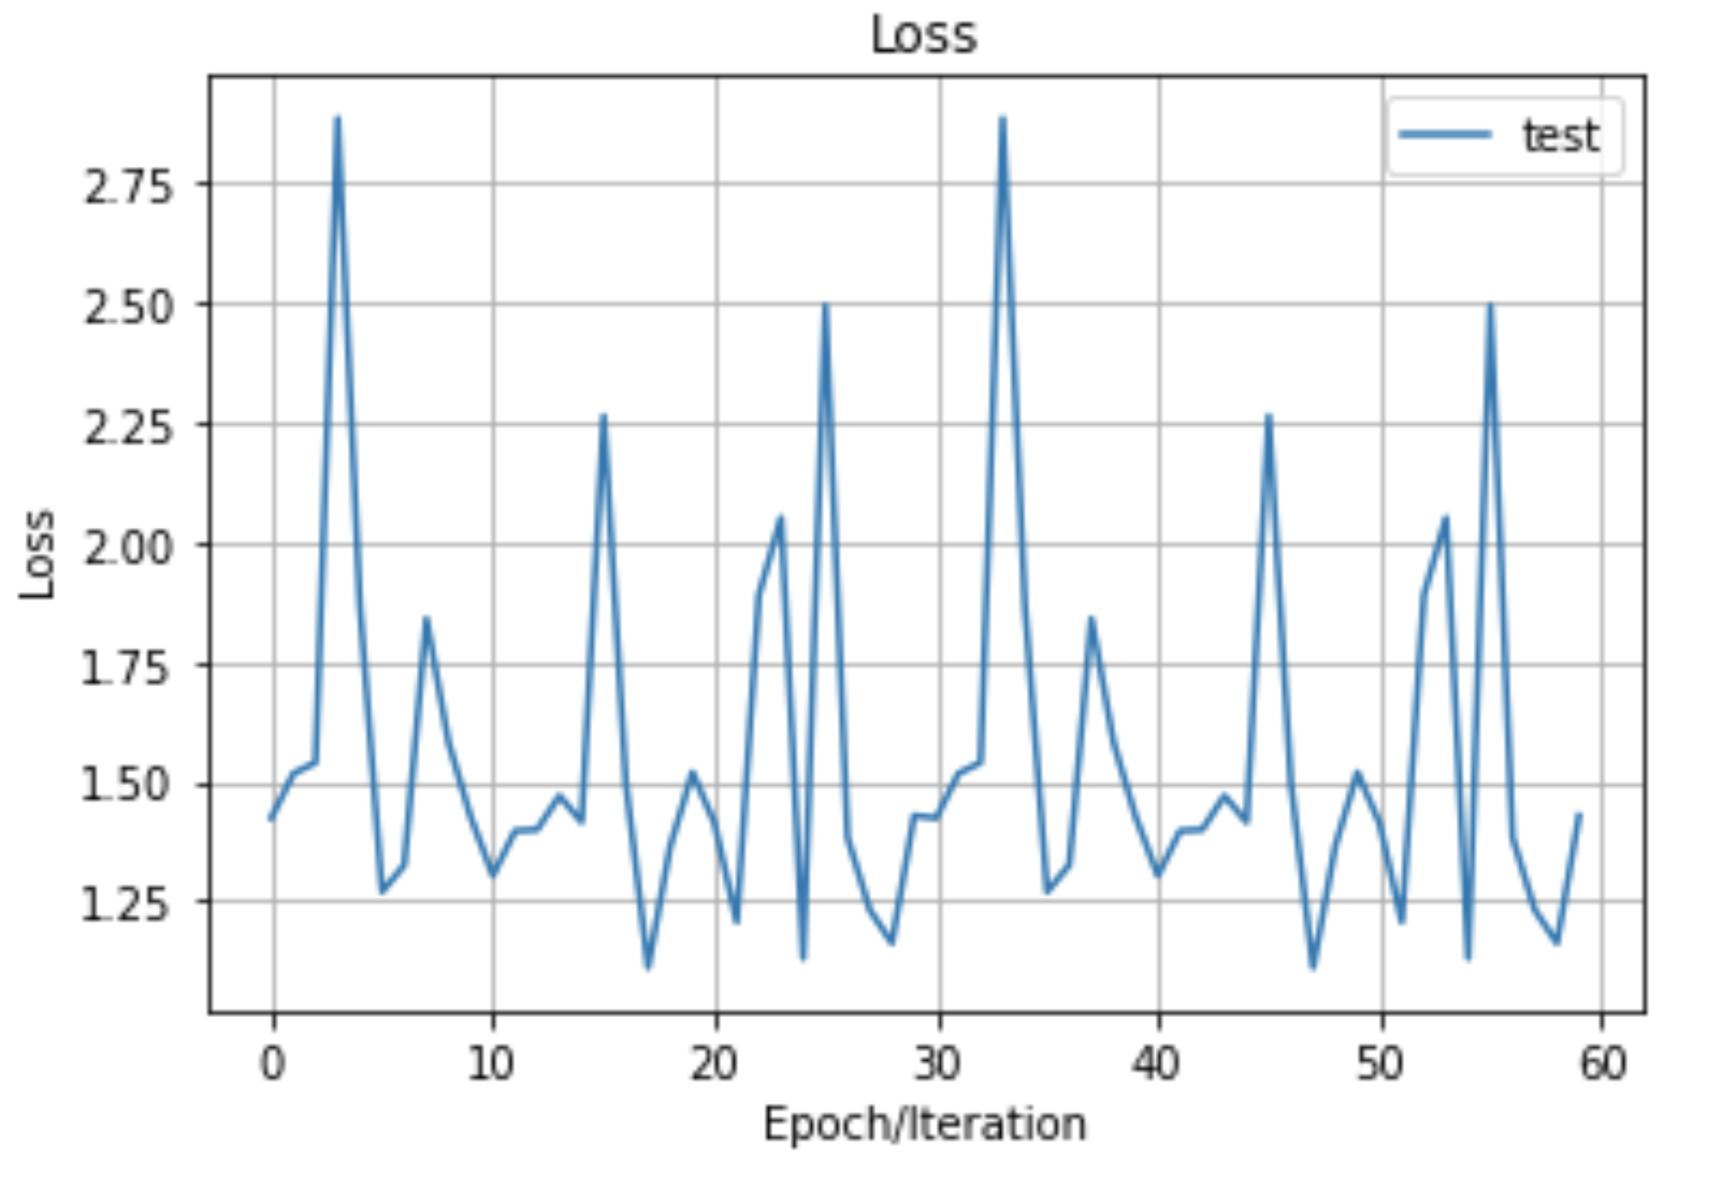
\includegraphics[width=1\linewidth]{images/losstest.png} \\ а)}
\end{minipage}
\hfill
\begin{minipage}[h]{0.49\linewidth}
\center{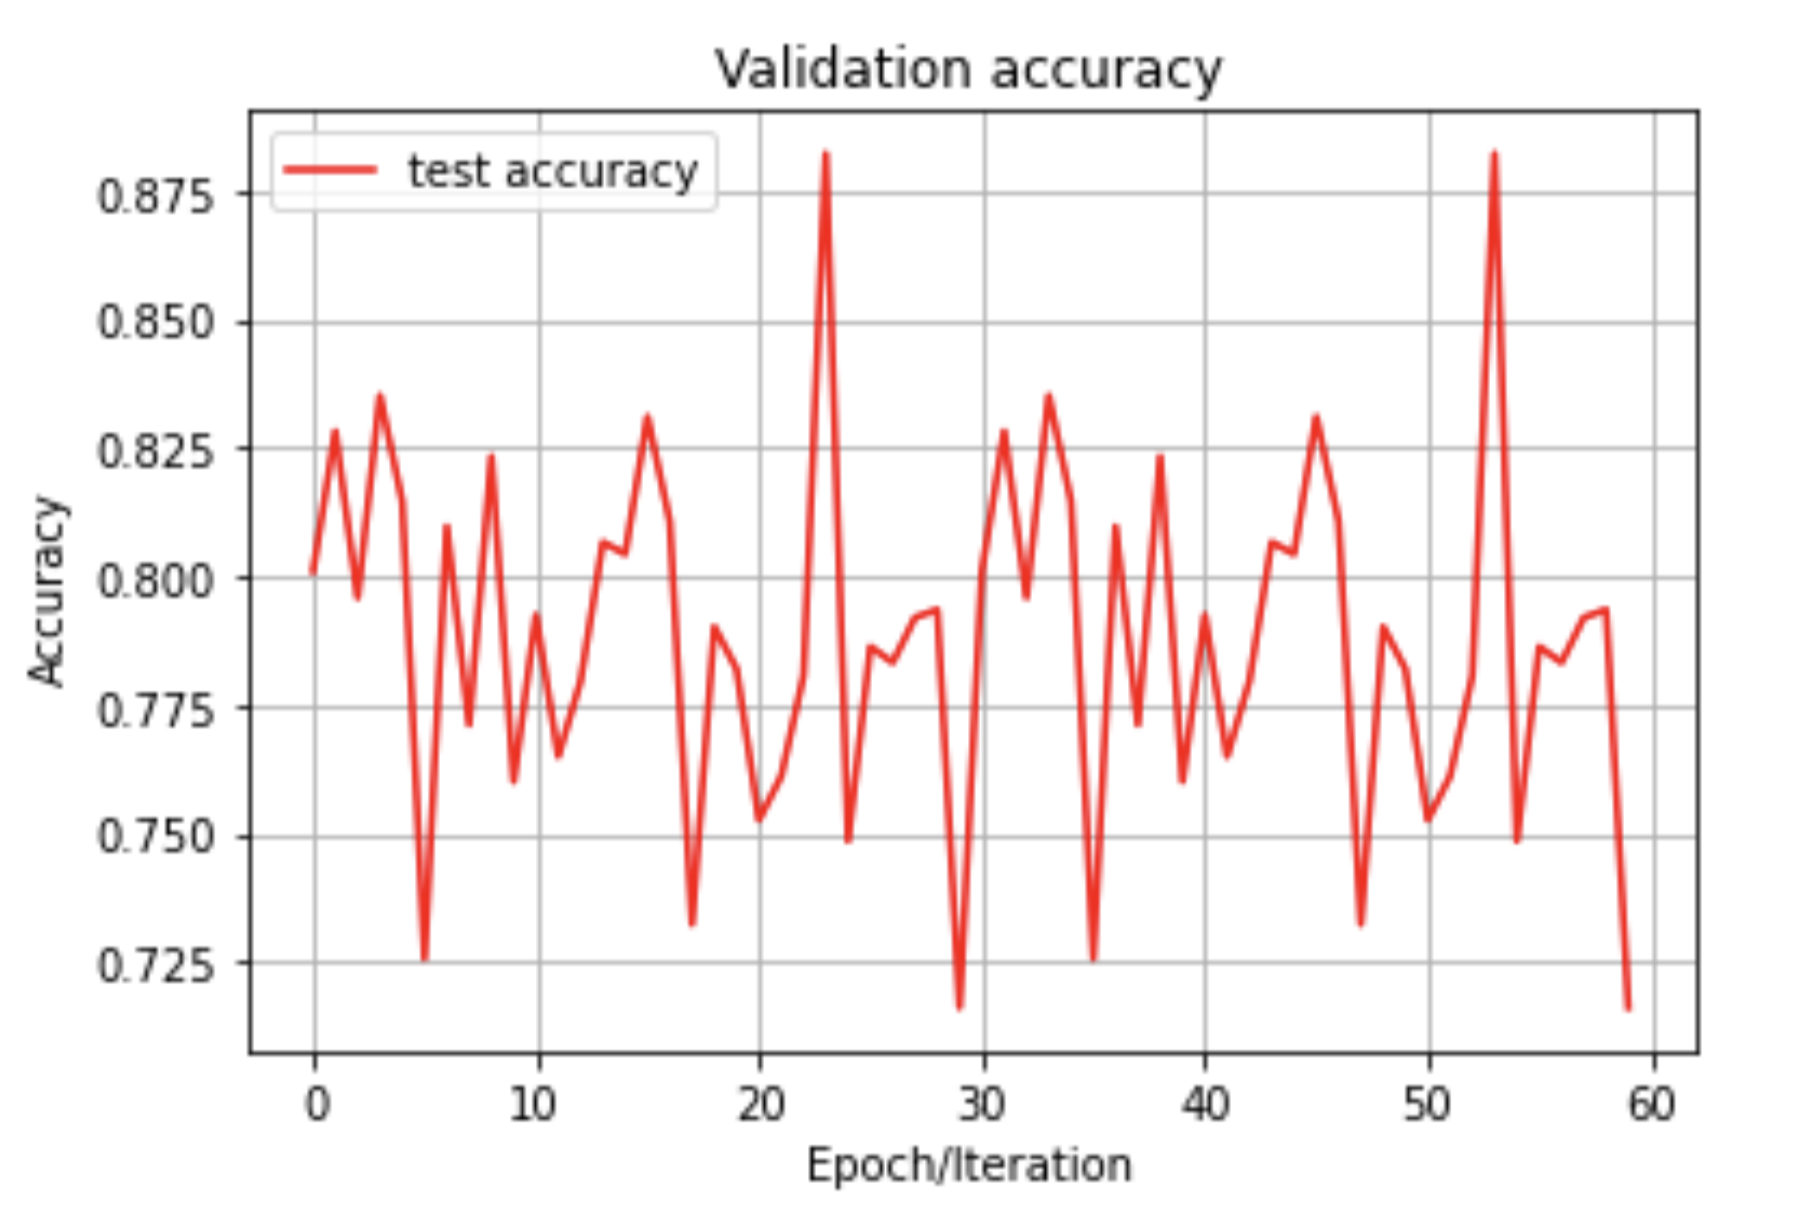
\includegraphics[width=1\linewidth]{images/valtest.png} \\ б)}
\end{minipage}
\caption{Процесс тестирования. а) график зависимости средней по данным MSE ошибки от эпохи; б) график зависимости средней по данным точности от эпохи.}
\label{test}
\end{figure}

Ошибка в среднем $1,56$ м$^2$ по траекториям.  А точности $5\%$ среднем мы достигаем в $79\%$  фильтрации.

\textbf{Вывод:} Сеть обучилась на наших данных, но возможен рост характеристик точности при  увеличении  обучающей вывборки и колличества весовых параметров.
 
\newpage
\section{Сравнительный анализ}
На данный момент мы  уже имеем фильтр Калмана и его новую версию, с применением  рекуррентной  нейронной сети.  Сравним результаты фильтраций траекторий полетов баллистических снарядов, уже привычными,  функциями MSE и Accuracy (из главы \hyperref[trainval]{Обучение  и валидация}).

\begin{figure}[h!]
\begin{center}
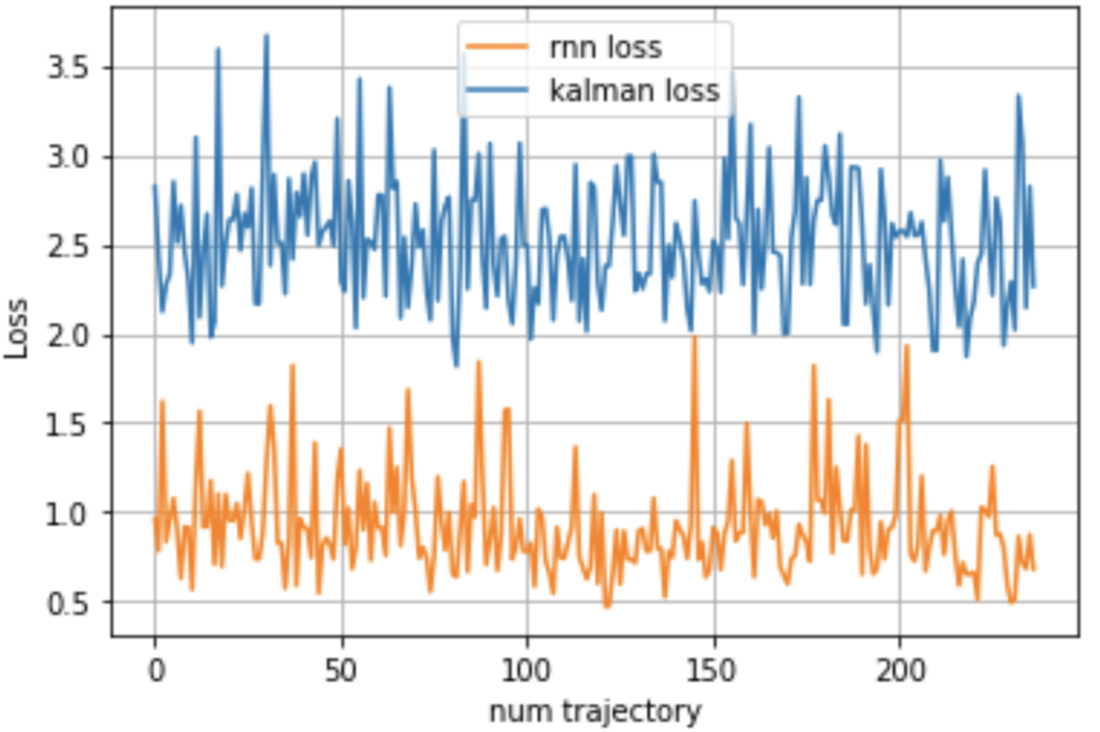
\includegraphics[width=0.6\textwidth]{images/battle1.png}
\end{center}
\caption{Средние MSE потери по траекториям} \label{battle1}
\end{figure}

Среднии по траекториям потери RNN фильтра Калмана составляют $0,9$ м$^2$,  тогда как у классического девяти-мерного фильтра они равны $2,5$ м$^2$.

\begin{figure}[h!]
\begin{center}
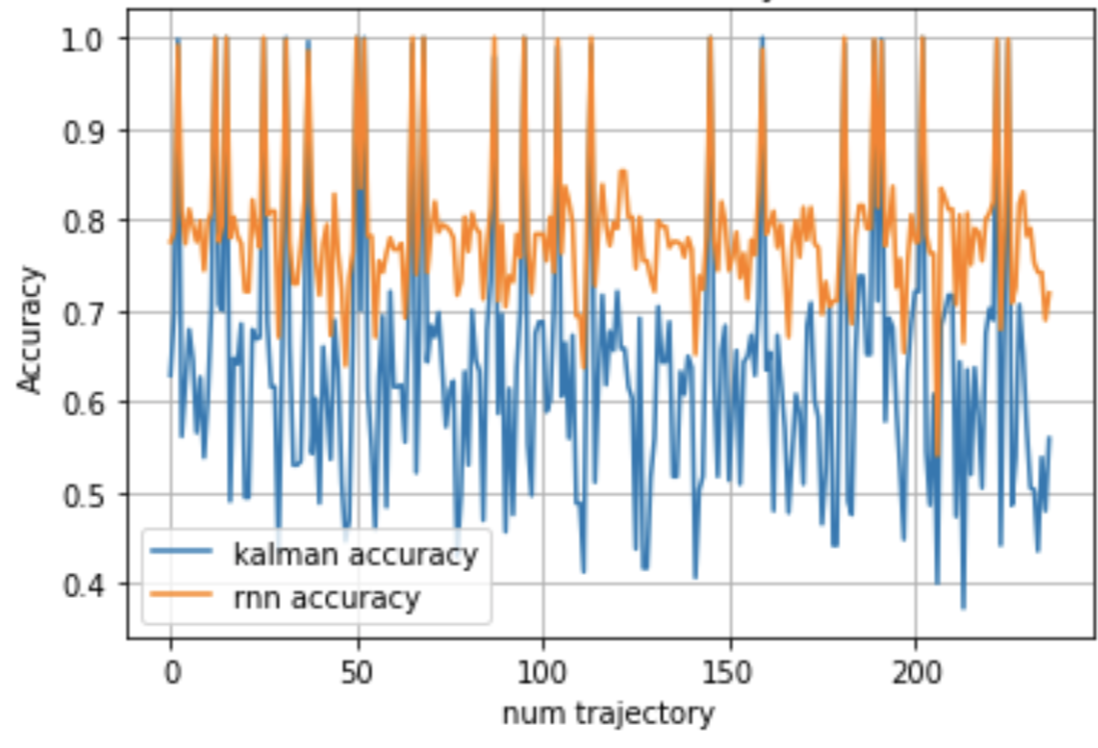
\includegraphics[width=0.6\textwidth]{images/battle2.png}
\end{center}
\caption{Средняя точность по траекториям} \label{battle2}
\end{figure}

В $5\%$-ую точность в среднем по траектории попадают $78\%$ результатов фильтрации RNN,  и $63\%$ для фильтра Калмана. 

Для исследования характеристик  фильтров, также рассмотрим их работу не в среднем, а на конкретной произвольной траекторие.  Будем выводить графики вида: |<<сигнал>>-<<сигнал+шум>>| и рядом |<<фильтрованный сигнал>>-<<сигнал+шум>>| в зависимостри от времени  (\textbf{в секундах}).

$$[t]=\text{сек};\qquad\qquad[x]=[y]=[z]= \text{м}.$$


 \begin{figure}[h]
\begin{minipage}[h]{0.49\linewidth}
\center{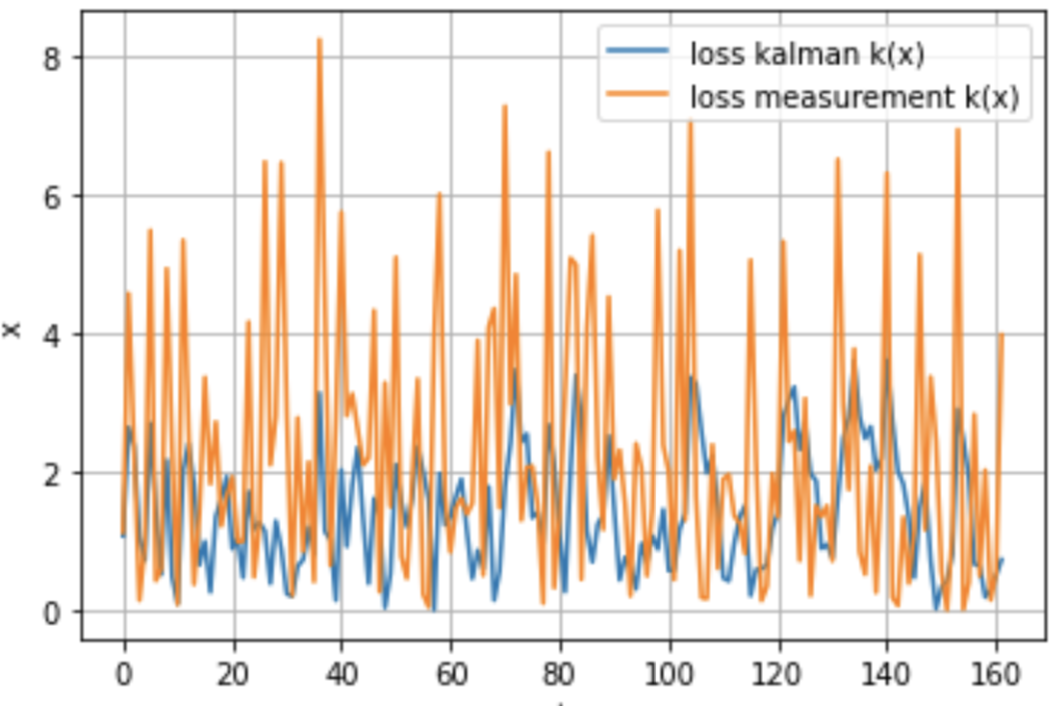
\includegraphics[width=1\linewidth]{images/kalmanx.png} \\ а)}
\end{minipage}
\hfill
\begin{minipage}[h]{0.49\linewidth}
\center{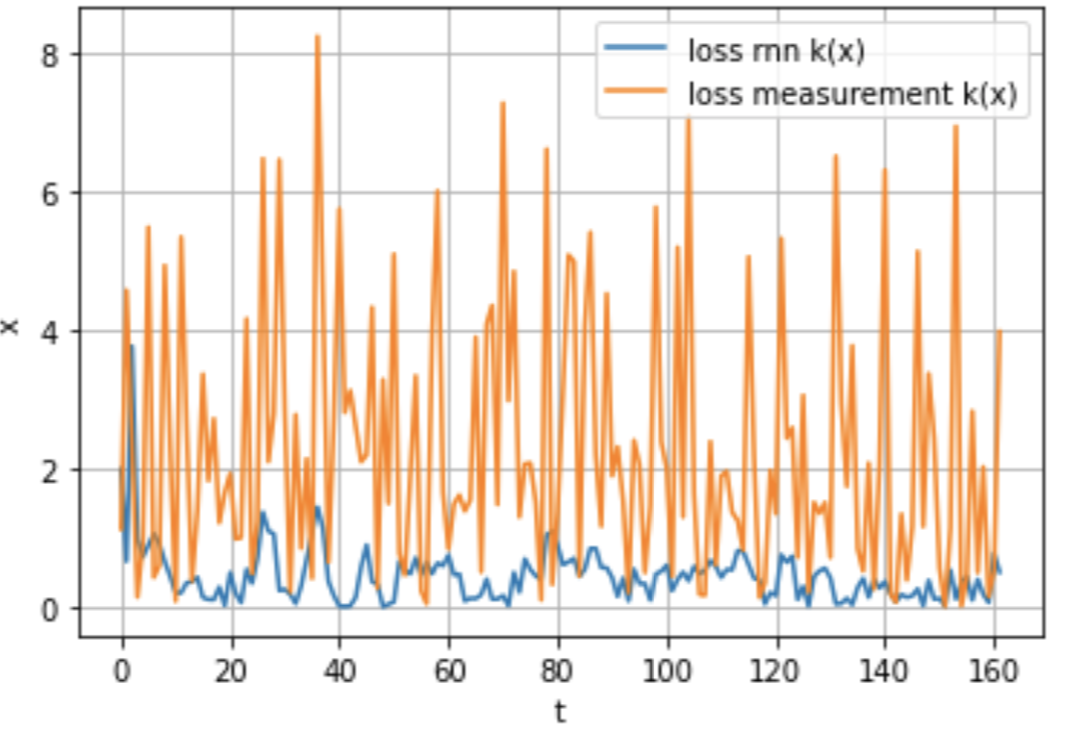
\includegraphics[width=1\linewidth]{images/nnx.png} \\ б)}
\end{minipage}
\caption{Графики ошибки по оси $x$. а) для классического фильтра Калмана; б) для фильтра Калмана с NN.}
\label{batlx}
\end{figure}

 \begin{figure}[h]
\begin{minipage}[h]{0.49\linewidth}
\center{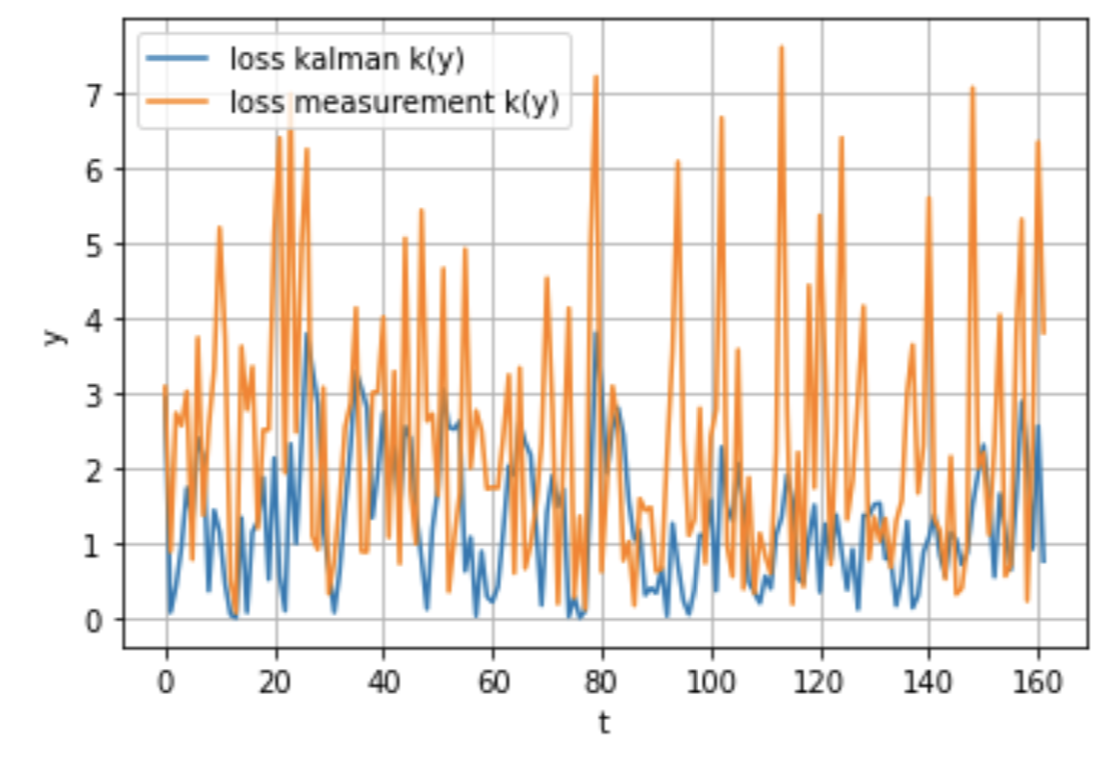
\includegraphics[width=1\linewidth]{images/kalmany.png} \\ а)}
\end{minipage}
\hfill
\begin{minipage}[h]{0.49\linewidth}
\center{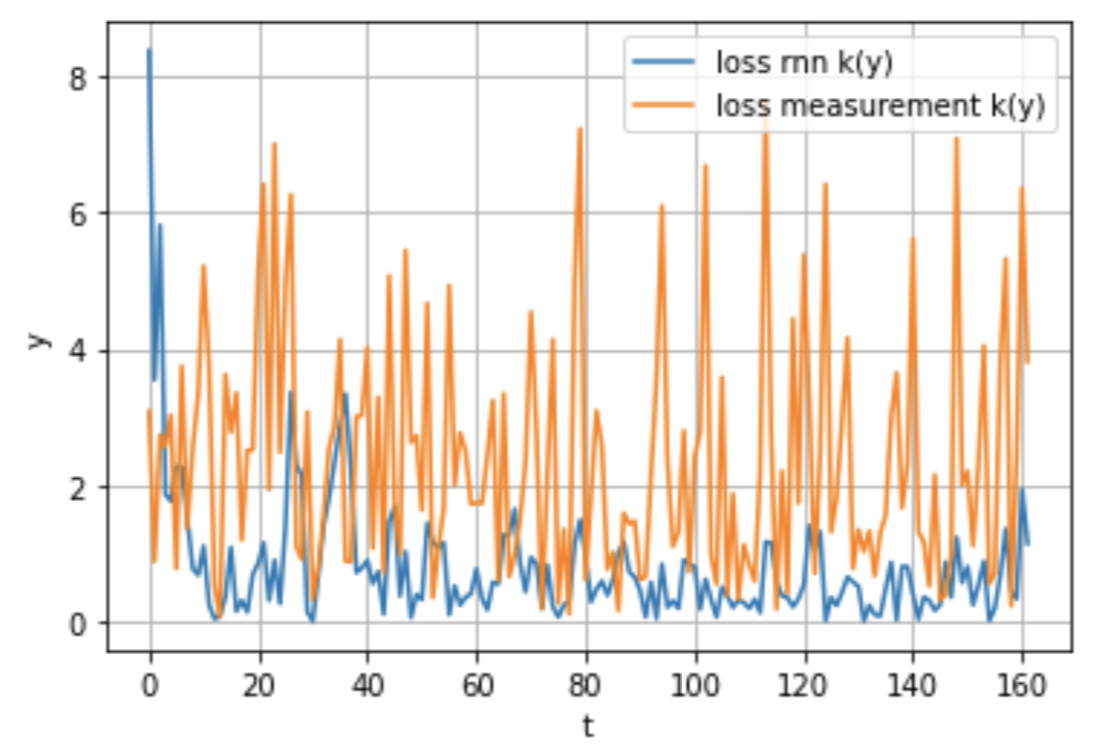
\includegraphics[width=1\linewidth]{images/nny.png} \\ б)}
\end{minipage}
\caption{Графики ошибки по оси $y$. а) для классического фильтра Калмана; б) для фильтра Калмана с NN.}
\label{batly}
\end{figure}

\newpage

 \begin{figure}[h]
\begin{minipage}[h]{0.49\linewidth}
\center{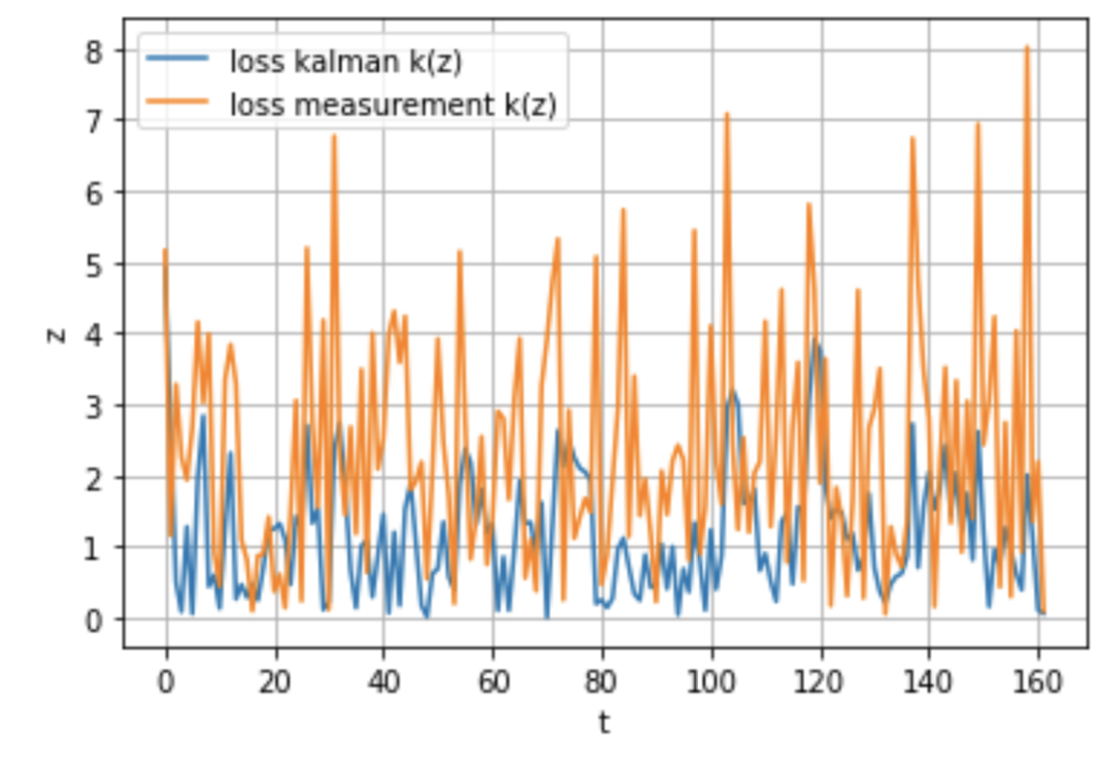
\includegraphics[width=1\linewidth]{images/kalmanz.png} \\ а)}
\end{minipage}
\hfill
\begin{minipage}[h]{0.49\linewidth}
\center{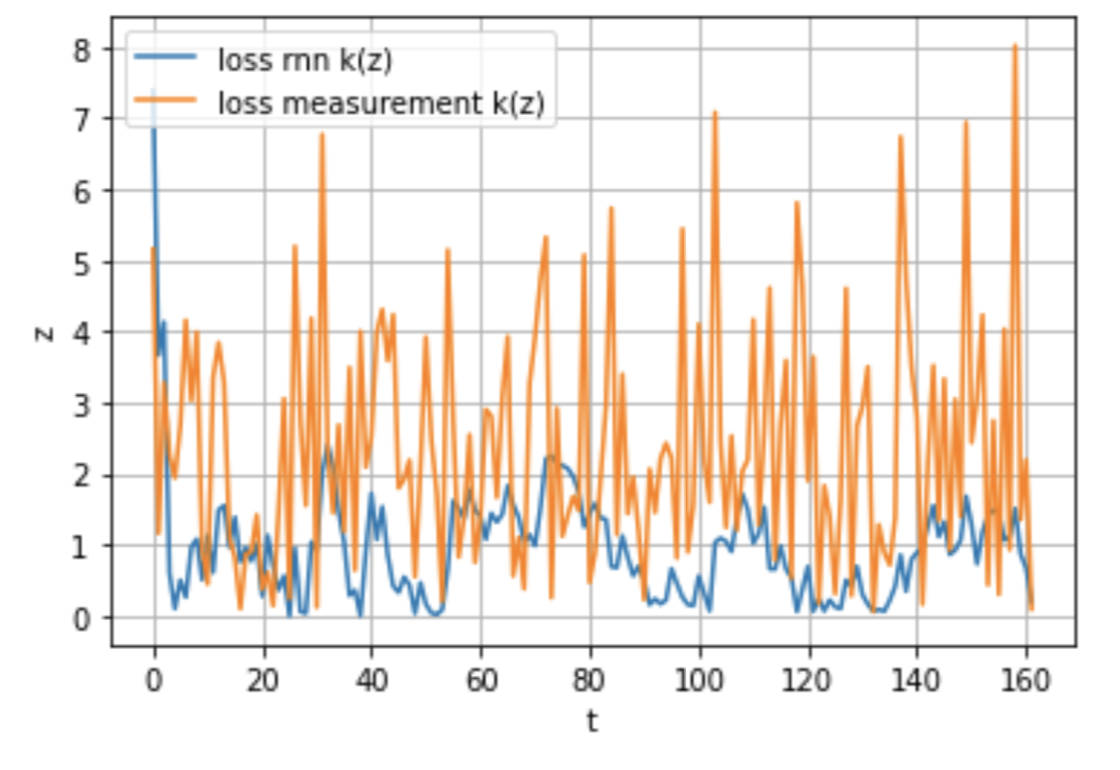
\includegraphics[width=1\linewidth]{images/nnz.png} \\ б)}
\end{minipage}
\caption{Графики ошибки по оси $z$. а) для классического фильтра Калмана; б) для фильтра Калмана с NN.}
\label{batlz}
\end{figure}

Из графиков видно, что ошибка фильтрации алгоритмом Калмана с нейронной сетью ниже, чем у классического.  Но из-за неверных предсказаний о первой координате, неточность у фильтра с NN в начале может быть выше, чем у стандартного фильтра.

Качественно  посмотрим  на  проекции траекторий на плоскостях $XY$, $XZ$, $YZ$:

\begin{figure}[h!]
\begin{center}
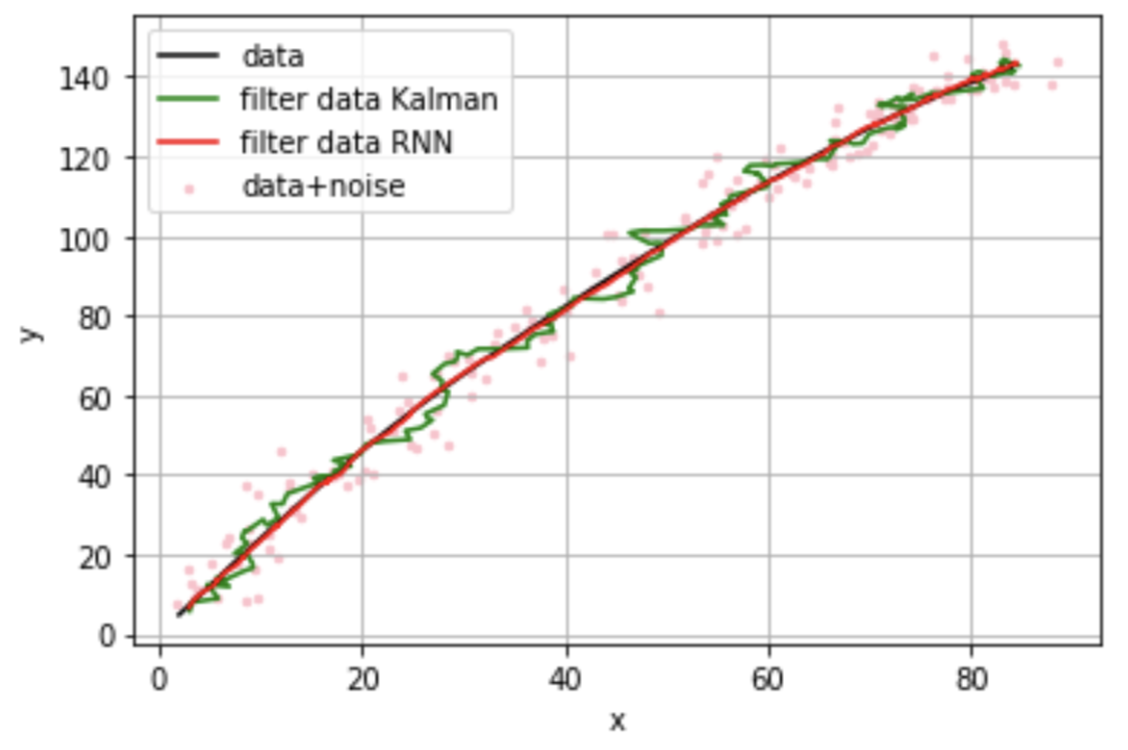
\includegraphics[width=0.7\textwidth]{images/xy.png}
\end{center}
\caption{Средняя точность по траекториям} \label{xy}
\end{figure}

\begin{figure}[h!]
\begin{center}
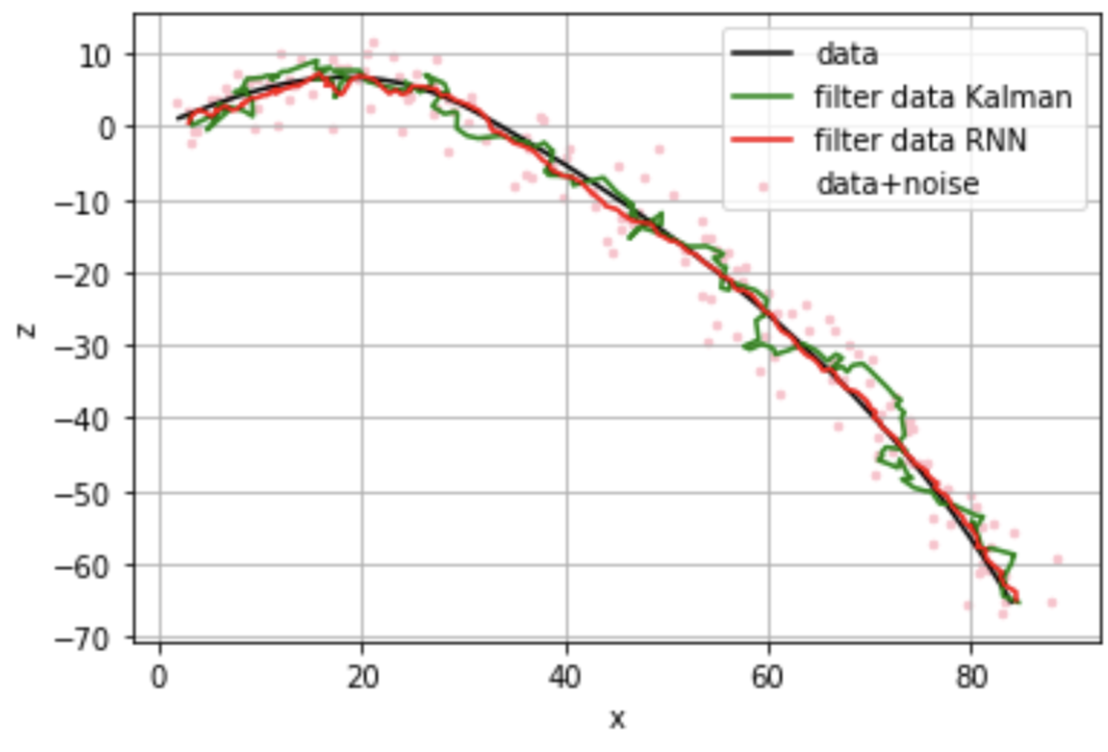
\includegraphics[width=0.7\textwidth]{images/xz.png}
\end{center}
\caption{Средняя точность по траекториям} \label{xz}
\end{figure}
\newpage
\begin{figure}[h!]
\begin{center}
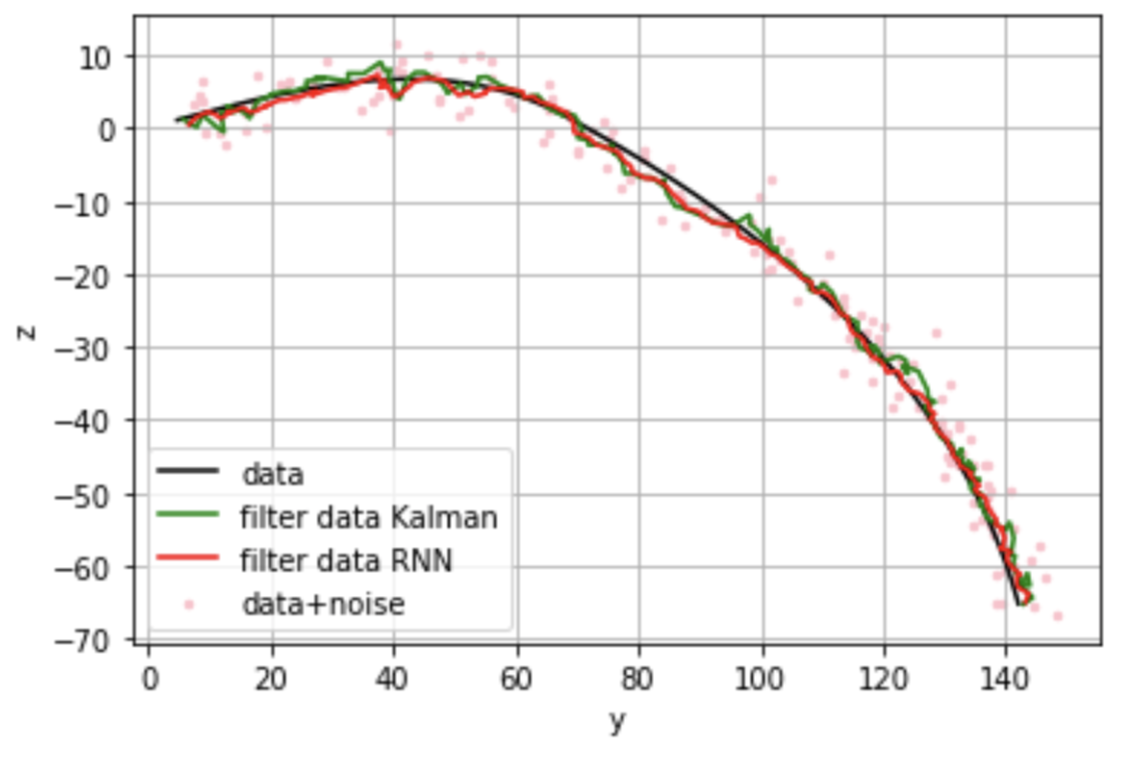
\includegraphics[width=0.7\textwidth]{images/yz.png}
\end{center}
\caption{Средняя точность по траекториям} \label{yz}
\end{figure}

Оба фильтра хорошо приблежают сигнал к истинному, но фильтр с нейронной сетью, полагаясь на <<память>>,  лучше обрабатывает траекторию, самотоятельно подстраиваясь под спектор шума.


\newpage
\section{Выводы}

\begin{itemize}
\item Исследовали и реализовали модель классического алгоритма  Калмана;
\item Изучили часть вопросов и проблем связанных с фильтрацией,   нашли решение в применение нейронных сетей к фильтру;
\item Разобрали теорию машинного обучения;
\item Написали работающую систему фильтра Калмана с рекуррентной нейронной сетью(LSTM);
\item Сравнили результаты двух моделей фильтров: 
\begin{itemize}
\item Среднии по траекториям потери RNN фильтра Калмана составляют $0,9$ м$^2$,  у классического девяти-мерного фильтра они равны $2,5$ м$^2$;
\item В $5\%$-ую точность в среднем по траектории попадают $78\%$ результатов фильтрации RNN,  и $63\%$ для фильтра Калмана;
\end{itemize}
\end{itemize}

Данная работа может найти свое применение и реализацию во многих сферах, связанных с обработкой сигналов. Она также требует улучшения и более глубокого изучения сравнения других отличительных характеристик фильтров.  

В планах на следующий семестр продолжить разарабатывать затронутую в отчёте тему, а именно:
\begin{itemize}
\item Улучшить архитектуру нейронной сети, чтобы увеличить её точность приближения;
\item Реализовать программное обеспечение для тестирования фильтра в полевых условиях на полигоне;
\item Провести более детальное сравнительное исследование различий в характеристиках.
\end{itemize}
\newpage
\section{Список литературы}
\renewcommand{\refname}{ }

	%\linenumbers
	\bibliographystyle{unsrt}
	\bibliography{thesis.bib}
	\begin{thebibliography}{7}
	\bibitem{KalmanPython} Книга Roger Labbe  \href{https://github.com/rlabbe/Kalman-and-Bayesian-Filters-in-Python}{ <<Kalman and Bayesian Filters in Python>>} 2014г;
	\bibitem{KalmanBook} Статья  R. E. KALMAN \href{http://www.cs.unc.edu/~welch/kalman/media/pdf/Kalman1960.pdf}{<<A New Approach to Linear Filtering and Prediction Problems>>} 1960г;
	\bibitem{nnkategor} Дипломная работа Фонарев А. Ю. \href{http://www.machinelearning.ru/wiki/images/9/99/Diploma_fonarev.pdf}{<<Машинное обучение с категориальными признаками.>>} 2014г;
	\bibitem{voron}  Курс лекций К. В. Воронцов \href{http://www.machinelearning.ru/wiki/images/6/6d/Voron-ML-1.pdf}{<<Математические методы обучения по прецедентам (теория обучения машин).>>};
	\bibitem{lasso}Книга Tibshirani, Robert  \href{https://www.researchgate.net/publication/228781252_Regression_shrinkage_and_selection_via_the_elastic_net_with_applications_to_microarrays}{<<Regression Shrinkage and Selection via the lasso>>} 1996г;
	\bibitem{Spokbook}Книга Spokoiny, Vladimir, Dickhaus, Thorsten <<Basics of Modern Mathematical Statistics>> 2015г;
	\bibitem{mtrixgrad}Методическое  пособие по вычислению матричных производных Justin Johnson <<Derivatives, Backpropagation, and Vectorization>> 2017г;
	\bibitem{ReLearning}Книга Richard S. Sutton and Andrew G. Barto <<Reinforcement Learning: An Introduction second edition>> 2018г;
	\bibitem{NN} Курс по машинному обучению МФТИ(НИУ)  \href{https://github.com/girafe-ai/ml-mipt}{<<Курс по машинному обучению.>> } 2014г;
	\bibitem{RNN} Лекция  7  \href{https://web.stanford.edu/class/cs224n/slides/cs224n-2019-lecture07-fancy-rnn.pdf}{<<Natural Language Processing with Deep Learning CS224N/ Ling28.>> } 2019г;
	\end{thebibliography}
	
\section{Приложение}
\label{appendix}

\end{document}
